\documentclass[11pt,a5paper,twoside]{book}
\usepackage{polyglossia}
\usepackage[a5paper]{geometry}
%\usepackage[utf8]{inputenc}%xelatex
\usepackage{tabu,longtable}
\usepackage{graphicx}
\usepackage{fancyhdr}
\pagestyle{fancyplain}
\usepackage{hyperref}
\hypersetup{
 pdftitle={GIMP 2.8.10},
 pdflang=nl
}
%  \newcommand{\url}[1]{\texttt{#1}}
%
\newcommand{\BETEREURL}[1]{\mbox{<\url{#1}>}}
\setdefaultlanguage{dutch}
\newcommand{\HRule}{\rule{\linewidth}{0.7mm}}
\author{Maxime Devos}
\title{GIMP}
%\makeindex{}
 \setmainfont[
  BoldFont={FreeSerifBold.otf},
  ItalicFont={FreeSerifItalic.otf},
  BoldItalicFont={FreeSerifBoldItalic.otf}
 ]{FreeSerif.otf}
 \setsansfont[
  BoldFont={FreeSansBold.otf},
  ItalicFont={FreeSansOblique.otf},
  BoldItalicFont={FreeSansOblique.otf}
 ]{FreeSans.otf}
 \setmonofont{FreeMono.otf}
% \renewcommand*{\ttdefault}{\familydefault}
\cfoot{}
\begin{document}
% \newcommand{\WEGindent}{\hspace*{20pt}}
 \newcommand{\sectie}[1]{\section{#1}}
 \newcommand{\nsectie}[1]{\section*{#1}}
 \newcommand{\subsectie}[1]{\subsection{#1}}
 \newcommand{\nsubsectie}[1]{\subsection*{#1}}
 \newcommand{\subsubsectie}[1]{\subsubsection{#1}}
 \newcommand{\nsubsubsectie}[1]{\subsubsection*{#1}}
 \newcommand{\XELATEX}{\mbox{X\raisebox{-0.5ex}{Ǝ}\LaTeX{}}}
 \newcommand{\XETEX}{\mbox{X\raisebox{-0.5ex}{Ǝ}\TeX{}}}
 \setlength{\parindent}{0pt}
 \newcommand{\GIMP}{GIMP}%\textsc{GIMP}}
 \addtolength{\columnsep}{1em}
 \setcounter{tocdepth}{3}
 \widowpenalty=100
 \clubpenalty=100
 \setlength{\parindent}{0pt}
 %Title page
 \frontmatter
 \begin{center}
 \HRule \\[0.4cm]
   \newlength{\gimptxtwidth} \newsavebox{\gimptxt} \savebox{\gimptxt}{%
   \huge{}\bfseries{}\GIMP{} 2.8.10}\settowidth{\gimptxtwidth}{\usebox{\gimptxt}}
   {
\includegraphics[width=\gimptxtwidth]{gimp-txt.pdf}\\[0.4cm]}
   \includegraphics{Wilber-head.png}\\[0.4cm]
   {\bfseries Nederlandse handleiding voor GNU Image Manipulation Program\\[0.4cm]}
 \HRule \\[1.5cm]
 \noindent
 \begin{minipage}[t]{0.4\textwidth}
  \begin{flushleft} \large
   \emph{auteur:}\\
    Maxime~Devos
  \end{flushleft}
 \end{minipage}%
 \begin{minipage}[t]{0.4\textwidth}
  \begin{flushright} \large
   \emph{uitgever:} \\
    Maxime Devos
  \end{flushright}
 \end{minipage}
 \vfill{}
 \today{}
\end{center}
%\twocolumn
\headheight=14pt
\newpage
 \rfoot{$%
          \frac{%
           \mbox{\thepage{}}%
          }{%
           \mbox{\pageref{EINDE}}%
          }$}
 \newsavebox{\GIMPBOX}\savebox{\GIMPBOX}{%
  %  \raisebox{0em}[0pt][0pt]{\makebox[0pt][l]{
   \includegraphics[height=3em]{e/gimp.pdf}
  %}}%
 }
 \lhead{\usebox{\GIMPBOX}}
\setotherlanguage{english}
 Copyright © 2015 Maxime Devos.\\
 Copyright © 2009 Hedwig Storch.\\
 Copyright © 2001 The Free Software Foundation.
 \textenglish{
  \paragraph{}Permission is granted to copy, distribute and/or modify this
  document under the terms of the GNU Free Documentation License, Version
   1.3 or any later version published by the Free Software Foundation;
  with no Invariant Sections, no Front-Cover Texts, and no Back-Cover Texts.
  A copy of the license is included in the section entitled “GNU Free Documentation License”.
 }
\sectie{Introductie}
 \GIMP{} is een programma om afbeeldingen mee te bewerken. De
  oorspronkelijke schrijvers van \GIMP{} zijn \mbox{Peter}~\mbox{Mattis}
  en \mbox{Spencer}~\mbox{Kimball}\footnote{%
  GNU Image Manipulation Program Gebruikershandleiding%
  }.
 U kunt \GIMP{} voor veel dingen gebruiken, zoals onvolmaaktheden in foto’s%
  verwijderen, tekeningen maken en zelfs logo’s%
  ontwerpen. Het is de bedoeling dat \mbox{deze} handleiding u
  op weg helpt met het \GIMP{}’en van afbeeldingen. Let wel op: we vertellen u niet
  alles over \GIMP{}. Als u een functie tegenkomt die hier niet beschreven staat:
  probeer het uit! De beste manier om te leren is wellicht trial and error: probeer
  en maak fouten. Indien het echt niet lukt, kunt u ook andere bronnen raadplegen.
 De website van \GIMP{} bevat hyperlinks naar informatie. De website van \GIMP{}
  bevindt zich op \footnote{\BETEREURL{%
   http://www.gimp.org/docs/%
  }}. De \GIMP{}-gebruikers%
  handleiding staat waarschijnlijk ook offline op uw computer, mischien wel
  als \footnote{/usr/share/gimp/2.0/help/nl/preface.html}?
\sectie{‘History’ Geschiedenis}
 \begin{longtabu} to \linewidth {X[0.7r] X[3,c] X[4,c] X[3,c]}
  jaar  &       naam          &
         titel        & uitgever\\\hline
  2001  &de artiesten van het Nevrax Design Team&
   Levitating, Meditating, Flute-playing Gnu by the Nevrax Design Team &
   the Free Software Foundation\\\hline
  2005  &    Janek Pfeifer    &
   Sarcophaga carnaria (Portugal2005)&
   Janek Pfeifer (via Wikimedia Commons)\\\hline
  2015  &     Maxime Devos    & 
      GIMP 2.8.10     & Maxime Devos\\\hline
 \end{longtabu}
 \addcontentsline{toc}{section}{0.3\space{}\space{}\space{}Inhoudsopgave}
 \tableofcontents{}
\mainmatter{}
\part{Gebruiken}
\chapter{Basiskennis}
 \sectie{Bestandsformaten}
  Er bestaan veel afbeeldingsbestandsformaten, sommigen meer bekend dan anderen.
  \begin{itemize}
   \item[naam] beschrijving
   \item[JPEG,] oftewel Joint Photographic Experts Group, comprimeert goed,
    maar verliest wel kwaliteit ‒ dit kwaliteitsverlies is niet goed
    zichtbaar bij foto’s ‒ en is populair bij huis-tuin-en-keukencamera’s,
    maar is niet geschikt voor afbeeldingen met tekst, geometrische figuren
    of diagrammen.
   \item[PNG,] Portable Network Graphics, comprimeert redelijk goed,
    ondersteunt zwart-wit- en en gedeeltelijke transparantie en
    verliest geen kwaliteit. Dat is handig voor schermafdrukken, logos en
    gameafbeeldingen. U kunt het ook gebruiken als u foto’s bewerkt en ze
    ondertussen moet delen met uw collega’s voor verdere bewerking. Zo
    voorkomt u gestapeld verlies van kwaliteit.\\
   \item[GIF,] ook wel bekend als Graphics Interchange Format is erg
    gelimiteerd in vergelijking met JPEG en PNG. Het ondersteunt slechts
    256 kleuren per afbeelding en comprimeert slecht. Maar, in vergelijking
    met JPEG en PNG heeft het toch een pluspunt: het kan voor bewegende
    afbeeldingen gebruikt worden.

   Er bestaan patenten op de comprimeermethode van GIF; sinds 2006 zijn
    ze allemaal verjaard\footnote{\BETEREURL{%
     http://www.gnu.org/philosophy/gif.html\#venuenote%
    }\\ het GNU Project}.
   \item[XCF] is hét bestandsformaat voor GIMP. Het ondersteunt lagen,
    transparantie, eenvoudige vectorgraphics en verschillende kleurmodi:
    8 bits per kanaal: rood, groen, blauw en alfa, geïndexeerd en
    grijswaarden.\\
   \item[SVG] is dan weer heel andere koek. SVG-afbeeldingen zijn
    vectorafbeeldingen, dat wil zeggen dat in plaats van met een raster te
    werken, er vormen worden gebruikt. Wanneer u met SVG werkt kunt u
    vectorvormen, afbeeldingen en tekst gebruiken. SVG’s kunnen interactief
    en dynamisch zijn\footnote{%
     \BETEREURL{http://www.w3.org/TR/SVG/intro.html\#AboutSVG}\\%
      World Wide Web Consortium, SVG 1.1 (second edition)%
     }.
  \end{itemize}
  \sectie{Kanalen}
  Kleuren krijgen in computers meestal een getal. Meestal worden ze
   onderverdeeld in meerdere delen, de \emph{kanalen}. Zo bestaan er o.a.
   de volgende:

  \begin{longtabu}{r|c|l}
   naam   &afkorting&subtractief (verf) of additief (licht)\\\hline
   rood   &    R    & licht\\
   groen  &    G    & licht\\
   blauw  &    B    & licht\\
   \hline
   cyaan  &    C    &subtractief\\
   magenta&    M    &subtractief\\
   geel   &    Y    &subtractief\\
   \hline
   alfa   &    A    &neutraal\\
  \end{longtabu}

  Alfa stelt de transparantie voor.

  Rood, groen en blauw kunnen natuurlijk ook subtractief gebruikt worden,
   en cyaan, magenta en geel additief, maar dat is minder gebruikelijk.
  Deze kanalen zijn niet alle kanalen die er bestaan, zo bestaat XYZ ook.
  Een combinatie van kanalen is een kleurenmodel.
  Het roodgroenblauw(alfa)kleurenmodel wordt veel gebruikt door computers en GIMP.
  Wanneer we het in dit boek hebben over een laag doelen we meestal op een rechthoek
   van pixels of vectorvormen.
 \sectie{Starten en stoppen}
  U kunt GIMP op meerdere manieren starten. Als u een desktopomgeving
   gebruikt en GIMP op uw computer heeft gezet met een packagemana%
   ger staat er waarschijnlijk een Wilbericoon op uw bureaublad of
   in een menu dat geopent kan worden met de SUPER-toets. Wilber is
   een coyote en staat op de cover van dit boek.

  U kunt het programma stoppen met het menu Bestand>Afsluiten.  
 \sectie{Maken, openen, opslaan en exporteren}
  We kunnen nu beginnen met afbeeldingen te maken, openen, opslaan
   en exporteren.
  \subsectie{Maken}
   Activeer het menu Bestand>Nieuw. Er verschijnt een venstertje waar u de
    afbeeldingsgegevens kunt invoeren. U kunt eventueel uit de
    sjabloonlijst een sjabloon kiezen.
   Bij afbeeldingsgrootte kunt u de grootte invoeren. Indien u een
    afbeelding wilt maken om die nadien af te drukken kunt u best
    uit het keuzemenu’tje een andere eenheid dan pixels kiezen.
   \\
   \\Verder kan ook de resolutie, de kleurenruimte, de ‘vulkleur’ en een opmerking
    aangepast worden. Open hiervoor ‘Geavanceerde opties’.
   Indien u een transparante achtergrond wilt, kunt u hiervoor ‘Transparantie’
    selecteren.
  \subsectie{Openen}
   Alreeds bestaande afbeeldingen kunnen geopend worden met Bestand>Openen.
   Dat menu-item opent een bestandskiezer waarmee u een afbeelding kunt kiezen.
  \subsectie{Opslaan}
   \GIMP{}’s autochtoon afbeeldingsbestandsformaat is XCF. Dus wanneer u
    een afbeelding opslaat wordt deze opgeslagen als XCF. Indien u dat niet
    wilt, moet u de afbeelding exporteren in plaats van op te slaan. Als u de
    afbeelding nog niet heeft opgeslagen, vraagt \GIMP{} naar de naam waarmee
    het opgeslagen moet worden.
  \subsectie{Exporteren}
   XCF wordt gebruikt door \GIMP{}, maar indien
    u uw afgewerkte afbeeldingen wilt gebruiken buiten \GIMP{} zult u ze eerst
    moeten exporteren naar een afbeeldingsformaat zoals PNG of JPEG.

   Kies hier voor het menu ‘Bestand>Exporteren als \ldots{}’. Er wordt een
    bestandskiesvenstertje geopend. Kies een afbeeldingsformaat uit de keuzelijst
    en activeer de knop ‘Exporteren’.
 \sectie{De GIMP-GUI}
 In figuur \begin{figure}%
   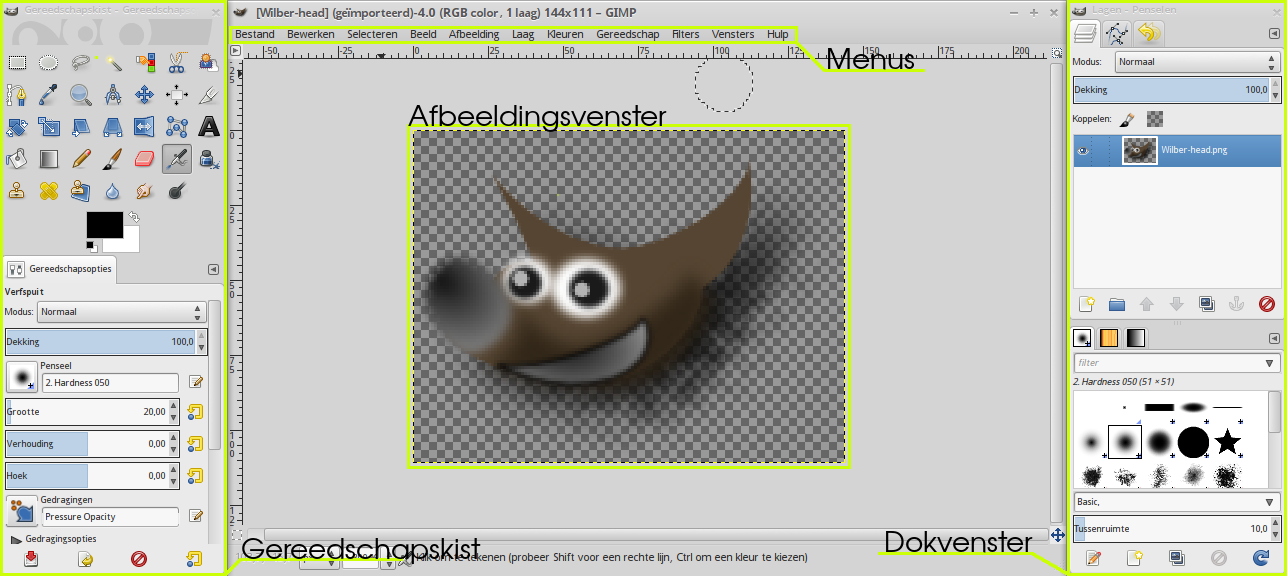
\includegraphics[width=0.90\linewidth]{GIMP-overview.png}%
   \caption{de \GIMP{}-GUI}\label{gx:overview}%
  \end{figure} \ref{gx:overview} ziet u
  de GUI van \GIMP{}. De GUI bevat een menubalk, een dokvenster en een
  gereedschapskist.
 \subsectie{Menubalk}
  De menubalk bevat menu’s en deze bevatten submenu’s. Door bepaalde menu-items
   te activeren kunt u opties omschakelen. De anderen zorgen voor een actie en
   openen meestal een venstertje waar om informatie wordt gegeven of gevraagd.
  \begin{itemize}
   \item Bestand bevat acties die rechtstreeks te maken hebben met bestanden,
    zoals openen, opslaan en exporten en afdrukken en verzenden.
   \item Bewerken bevat enkele eenvoudige bewerkacties, zoals knippen en
    plakken en voorkeuren.
   \item Selecteren heeft menu-items om de selectie mee te bewerken.
   \item Beeld past de afbeelding niet aan, maar hiermee kunt u wel het ‘beeld’
    aanpassen: weergavefilters, selectie, raster, volledig scherm \ldots{}
   \item Afbeelding biedt menu-items aan voor enkele ‘grove’ bewerkingen:
    de kleurmodus veranderen, horizontaal en verticaal spiegelen, 90 en 180
    graden draaien, vergroten en verkleinen en bijsnijden.
   \item Met Laag kunt u lagen maken, dupliceren
    en verwijderen, verankeren, samenvoegen, een alfakanaal of masker toevoegen,
    −180, −90, 90 en 180 graden draaien,
    spiegelen en bijsnijden.
  \end{itemize}
 \subsectie{Gereedschapskist}
  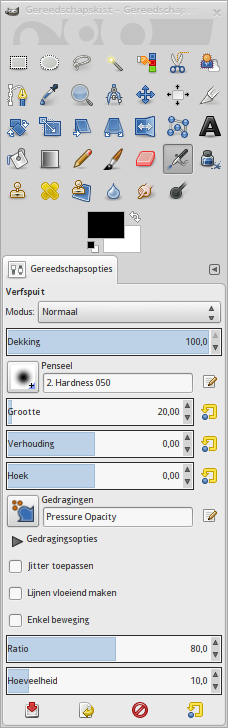
\includegraphics[height=\linewidth,angle=90]{gui/gereedschapskist.png}
  Links ziet u de gereedschapsiconen.
  Ten eerste zorgen het rechthoekje, de ovaal en de lasso respectievelijk
   voor een rechthoekige, ovaalvormige en vrije selectie. Daarnaast
   selecteert de toverstaf de pixels naast de aangewezen pixel die op
   de pixel lijken. Bovendien selecteert de driekleurenbalk-met-☝ alle
   pixels met ongeveer dezelfde kleur. Wat ook niet vergeten mag worden
   is de schaar die een ‘slim’ selectiegereedschap is: ze herkent
   vormen automatisch en past zich er aan aan. Met het hoofd-met-lichaam
   kunt u eenvoudig voorgrondobjecten selecteren. Met de pen worden
   paden getekend en aangepast. Het pipet
   ‘neemt kleuren op’: kiest kleuren. Het vergrootglas verandert het
   zoomniveau. De passer meet afstanden en hoeken. De multipijl wordt
   gebruikt om ‘lagen, selecties en andere objecten’ mee te verplaatsen.
   %uitlijnen laten we over
  Het mes snijdt lagen of de hele afbeelding bij. De volgende vijf
   blauwe icoontjes stellen respectievelijk draaien, schalen, hellen,
   perspectief en spiegelen voor. De zwarte hoodletter a wordt gebruikt
   voor het toevoegen van tekst aan afbeeldingen. De verfpot vult de
   selectie of de ‘gelijkende’ kleuren met een vaste kleur of een patroon.
  Het kleurenverloop zorgt voor een kleurenverloop.
  Deze hoeven niet altijd linear te zijn. Het potlood tekent vrije vormen
   met scherpe randen en het penseel tekent vloeiende lijnen. Het roze
   dekentje is een gum. De verfspuit is een penseel met variabele druk en
   met de inktpot kan men tekenen in calligrafische stijl. Met de stempel
   kunnen delen van de afbeelding gestempeld worden. De stempel met een
   perspectiefvlak kloont en past tegelijkertijd het perspectief aan.
  De waterdruppel is een penseel dat vervaging tekent. De vinger ‘smeert’
   de afbeelding uit, zoals u wellicht ook boter uitsmeert op boterhammen.
  Tenslotte maakt het zwartethermometeronderstuk delen van de
   afbeelding lichter of donkerder.

  Dat zijn in het totaal 34 gereedschappen.
  \subsubsectie{Gereeedschapsopties}
   Elk gereedschap heeft \textit{opties}. Deze veranderen de werking van het
    gereedschap.
\chapter{Foto’s}
 \sectie{Correctie}\label{ding:correctie}
  \GIMP{} heeft gereedschappen om onvolmaaktheden in foto’s mee te bewerken.
   Deze zijn er niet altijd voor bedoeld, maar ze werken wel.
  \subsectie{Rode ogen}\label{ding:rode ogen}
   Eerst moet u de ogen selecteren. U kunt hiervoor de \textit{lasso}
    gebruiken. Klik eerst op het icoon en maak daarna een rondje rond een oog
    terwijl u de linkermuisknop ingedrukt houdt (%
    \begin{figure}
     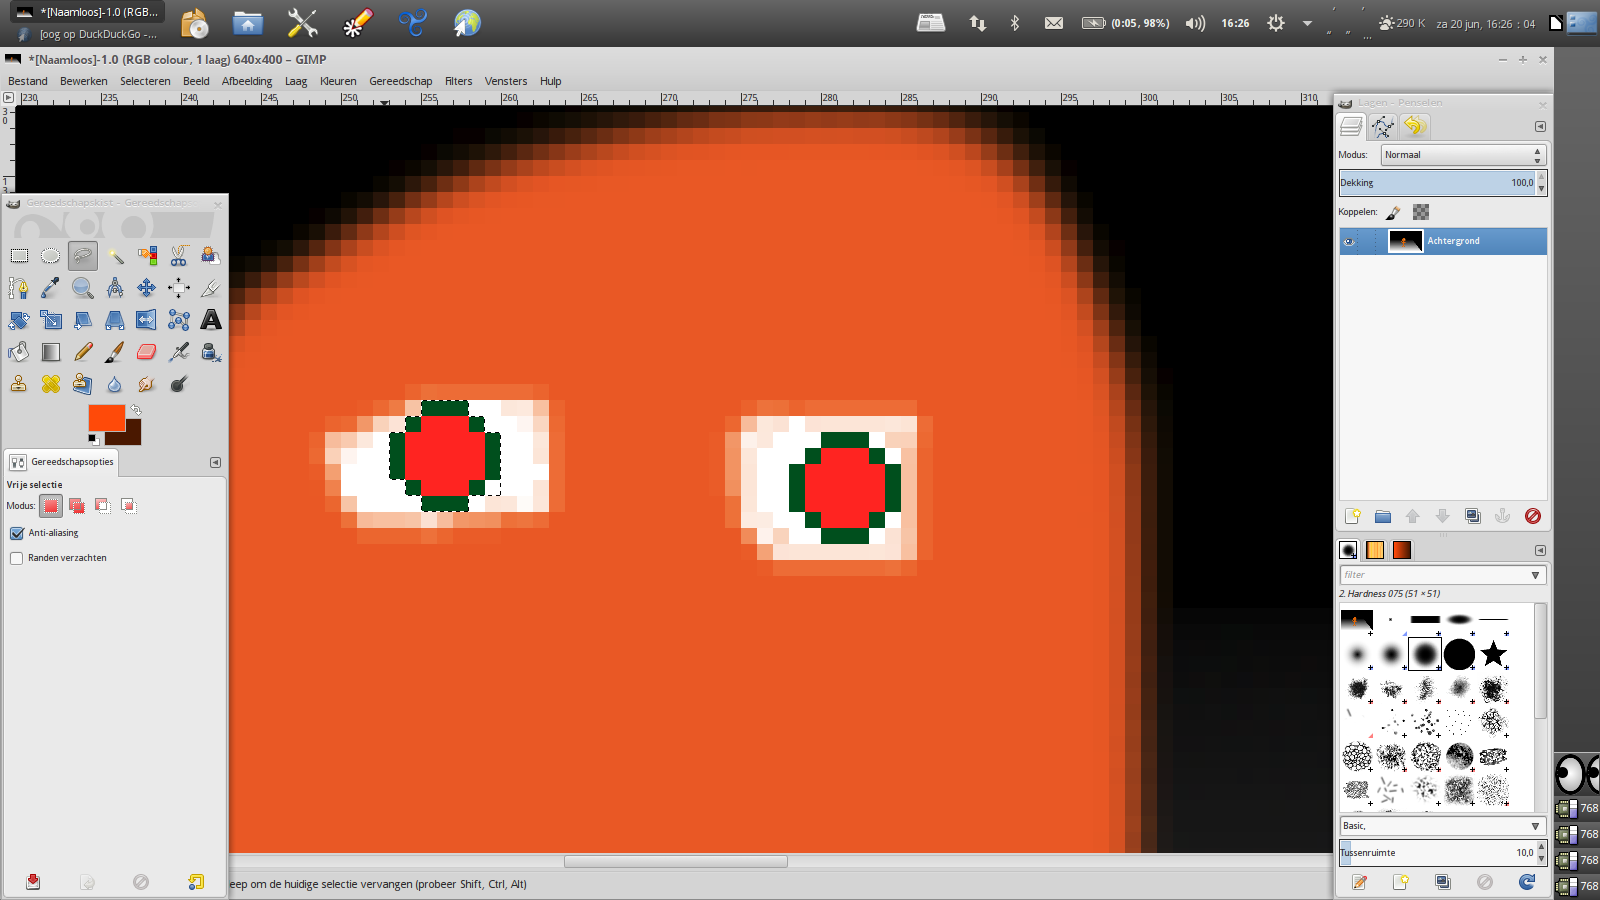
\includegraphics[width=0.90\linewidth]{redeyes/1.png}
     \caption{rode ogen verwijderen: stap 1}\label{gx:redeyes/1}%
    \end{figure}).

   Doe dit opnieuw met het rechteroog, maar houdt deze keer ook de ⎈-toets (%
    ⎈ is het ISO-toetsenbordsymbool voor control)
    ingedrukt. Met de ⎈-toets wordt de nieuwe selectie opgeteld met de oude selectie.

   Klik nu op het menu-item ‘Filters>Versterken>Rode ogen verwijderen…’ (%
    \begin{figure}
     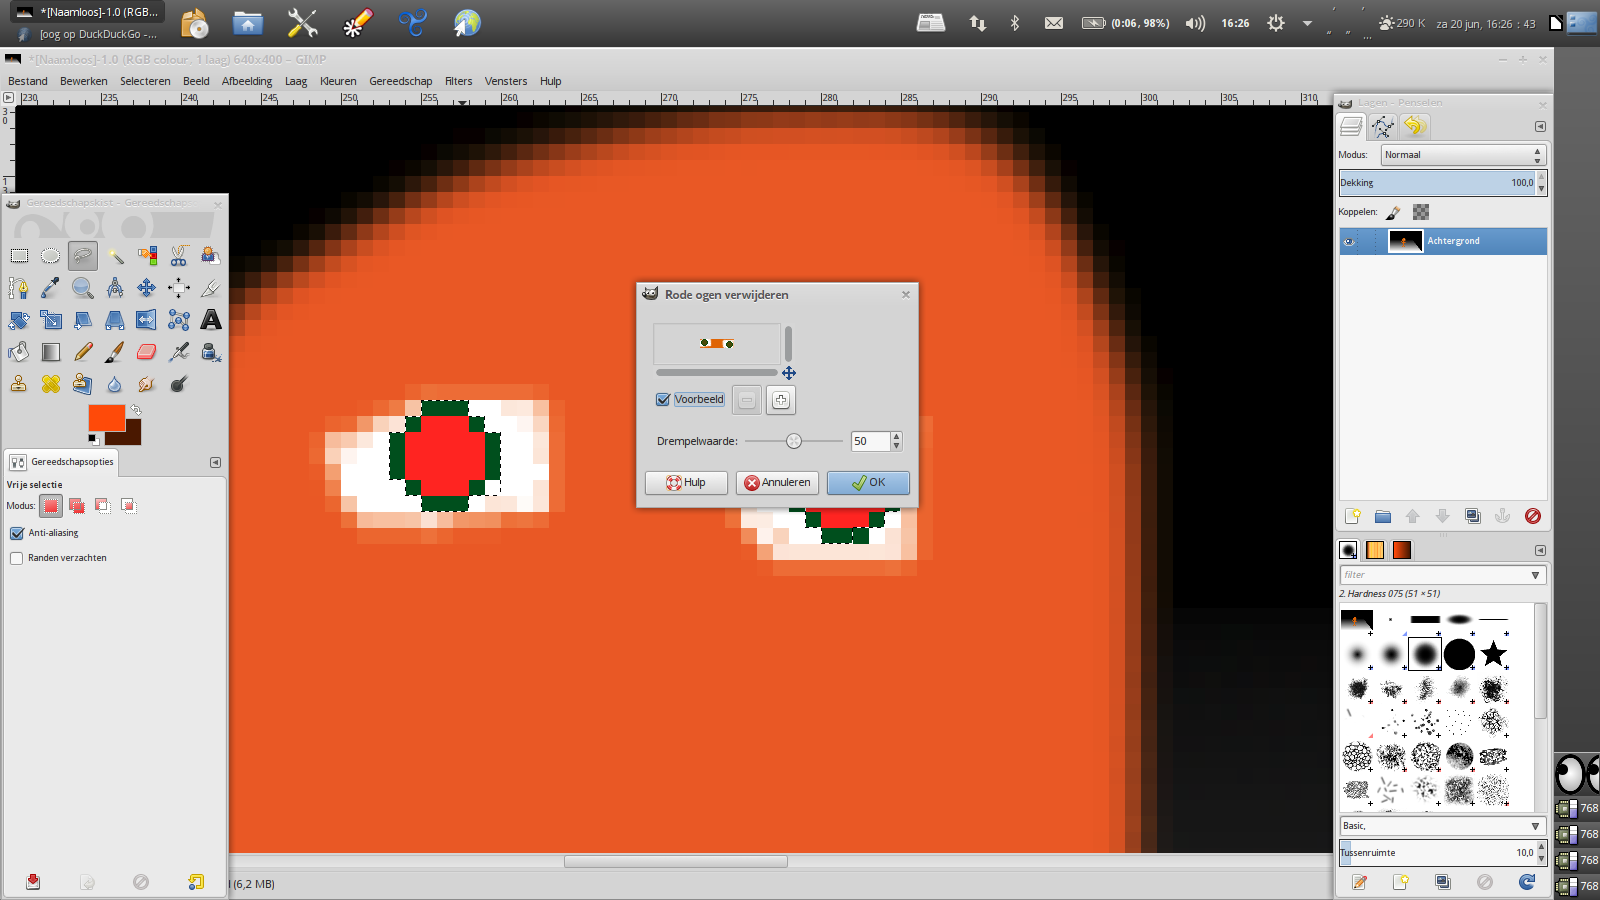
\includegraphics[width=0.90\linewidth]{redeyes/2.png}
     \caption{rode ogen verwijderen: stap 2}
     \label{gx:redeyes/2}%
    \end{figure}\ref{gx:redeyes/2}
    ) en daarna op √OK.

   U kunt het resultaat zien bij figuur \begin{figure}
    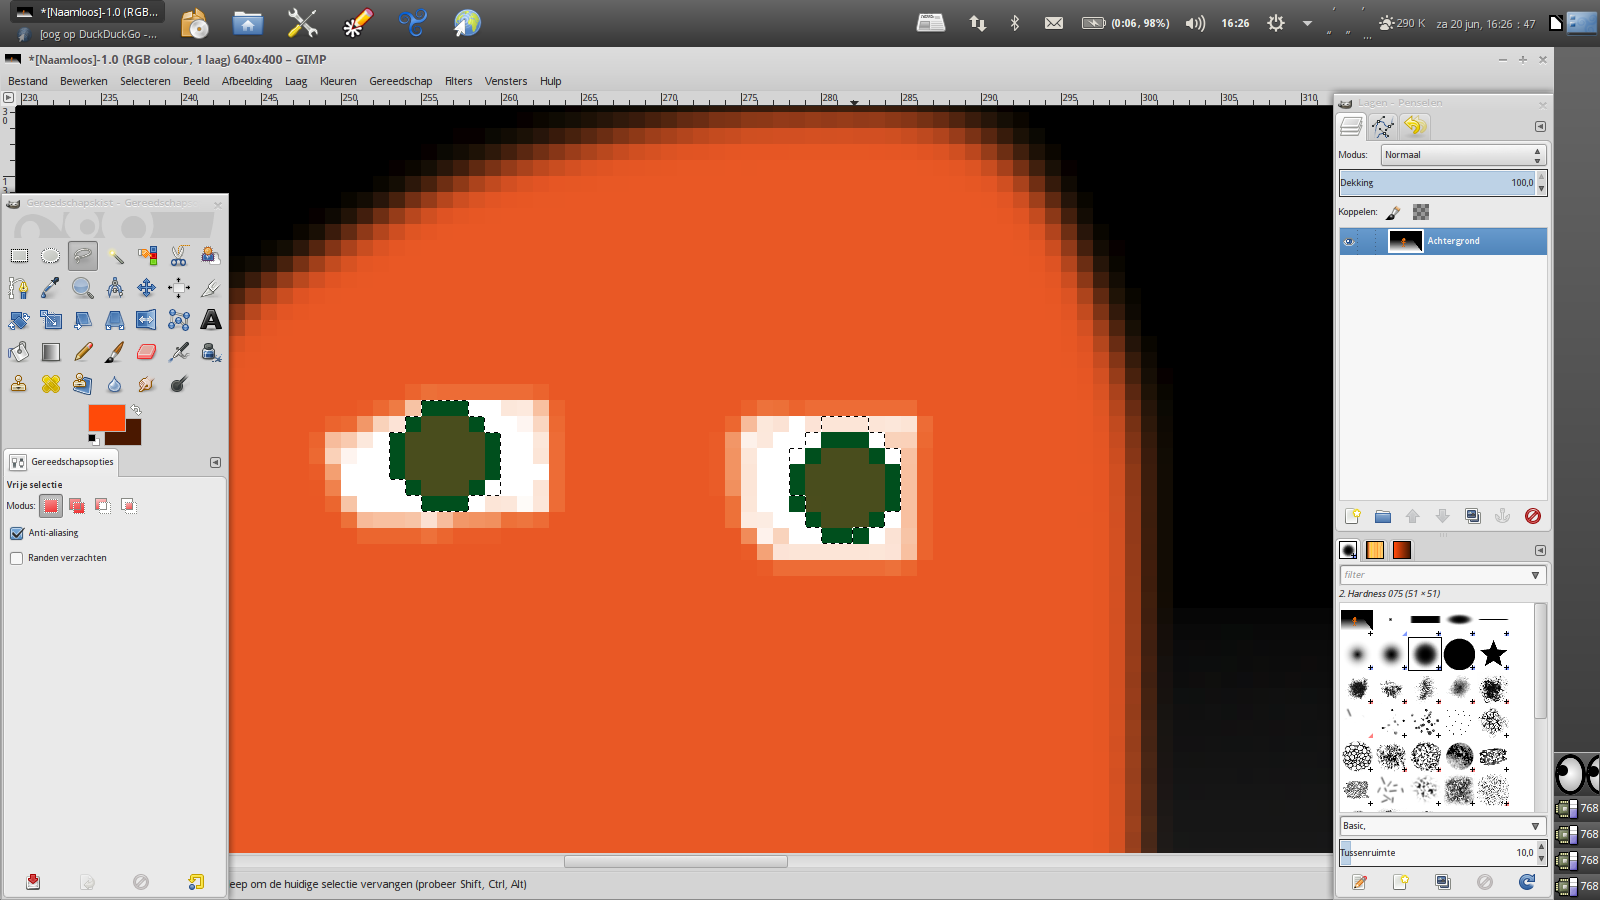
\includegraphics[width=0.90\linewidth]{redeyes/3.png}
    \caption{rode ogen verwijderen: het eindresultaat}
    \label{gx:redeyes/3}
   \end{figure}\ref{gx:redeyes/3}.
  \subsectie{Rimpels}
   \GIMP{} kan ook gebruikt worden voor het wegwerken van rimpels,
    tenminste, die op de foto’s, niet de echte. Voor de echte hebt
    u een plastisch chirurg nodig.

   Een van de manieren om dit te doen is \textit{stempelen}. Huid zonder
    rimpels wordt gekopieerd en geplakt op huid met rimpels.

   Vindt eerst een goede reden vooraleer foto’s op deze manier te bewerken:
    deze manipulatie tast de authenticiteit aan en misleidt het publiek.
%   De benodigde, goede redenen zijn schaars, mischien zelfs niet-bestaand.
   \begin{itemize}
    \item[1.]
     Open het venster ‘Editor Selecties’. Dat kan gedaan worden met
      het menu-item ‘Selecteren>Editor Selecties’.
    \item[2.]
     \begin{figure}
      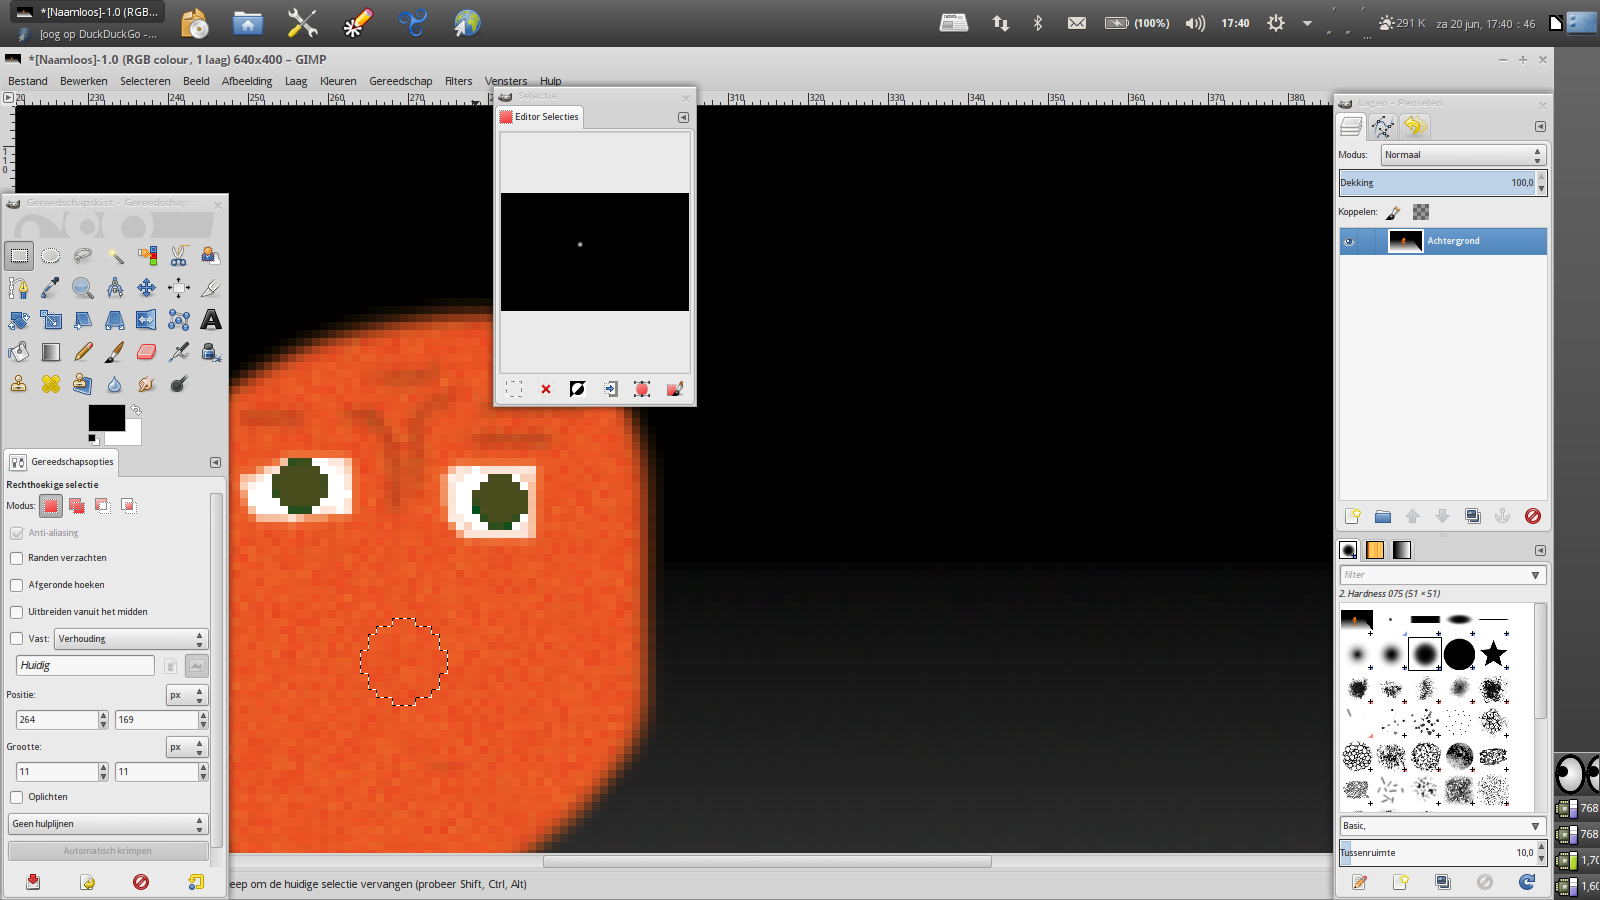
\includegraphics[width=0.9\linewidth]{rimpels/2.png}
      \caption{rimpels wegwerken}
      \label{gx:rimpels/2}
     \end{figure}\ref{gx:rimpels/2}%
      : Selecteer een stuk rimpelloze huid. Activeer daarna het
      menu-item ‘Selecteren>Selectieranden verzachten…’ en druk
      op √OK. Herhaal dat tot de randen van het wit in het
      selectiekader er vaag uitzien.
    \item[3.] Kopieer\marginpar{⎈+C} het geselecteerde
      deel van de laag.
     Plak\marginpar{⎈+V} het en versleep het naar een
      plek met rimpels. Nadat het geplakt is kunt u best
      de ‘Zwevende Selectie’ verankeren\marginpar{⎈+H}.
    \item[4.]
     Herhaal het plakken, verslepen en verankeren totdat de
      rimpels weg zijn.
    \item[5.]
     \begin{figure}
      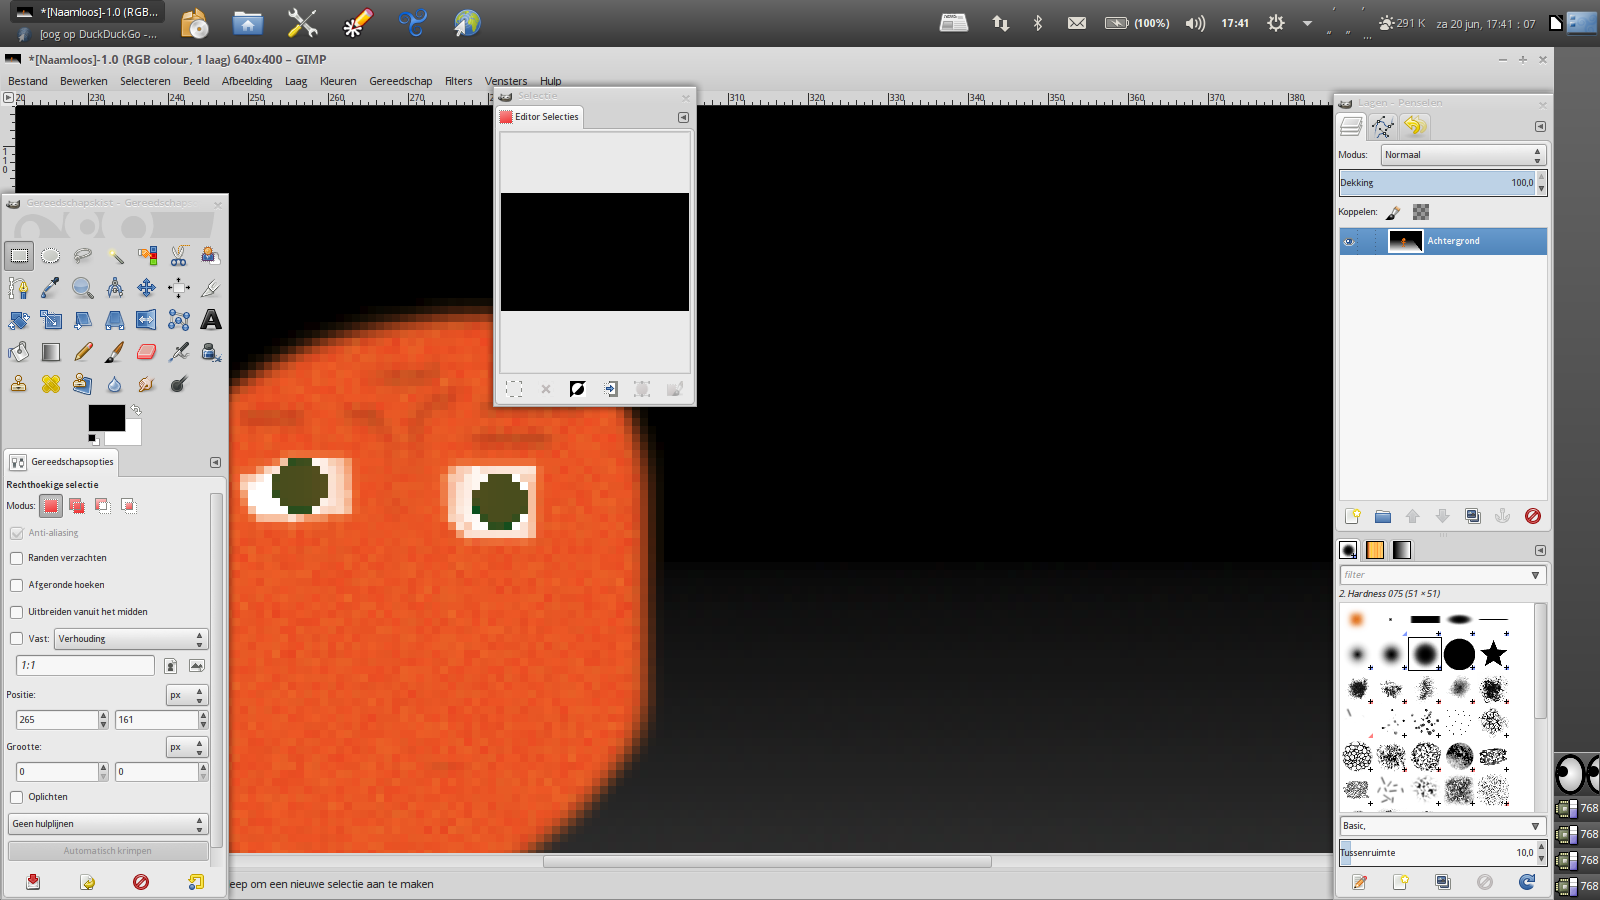
\includegraphics[width=0.90\linewidth]{rimpels/3.png}
      \caption{rimpels wegwerken}
      \label{gx:rimpels/3}%
     \end{figure}\ref{gx:rimpels/3}%
      : Bewonder of verafschuw het resultaat.
   \end{itemize}
  \subsectie{Kleurencurves}
   Indien de foto te weining of te veel blauw, groen, rood of
    doorzichtigheid heeft kunt u ‘kleurcurves’ gebruiken.
   \begin{figure}
    \centering
    \setlength{\unitlength}{1.3cm}
    \begin{picture}(5,1)
%     \thicklines
     \qbezier(0,0)(3,0)(5,1)
%     \thinlines
     \put(0,0){\line(0,1){1}}
     \put(5,0){\line(0,1){1}}
     \put(0,1){\line(1,0){5}}
     \put(0,0){\line(1,0){5}}
    \end{picture}
    \caption{een curve}
   \end{figure}
   Alle kleurenwaarden van de pixels worden de y-waarde op de curve.
   \begin{itemize}
    \item[1.] Activeer het menu-item ‘Kleuren>Curves…’
    \item[2.]
     \begin{figure}
      \centering
      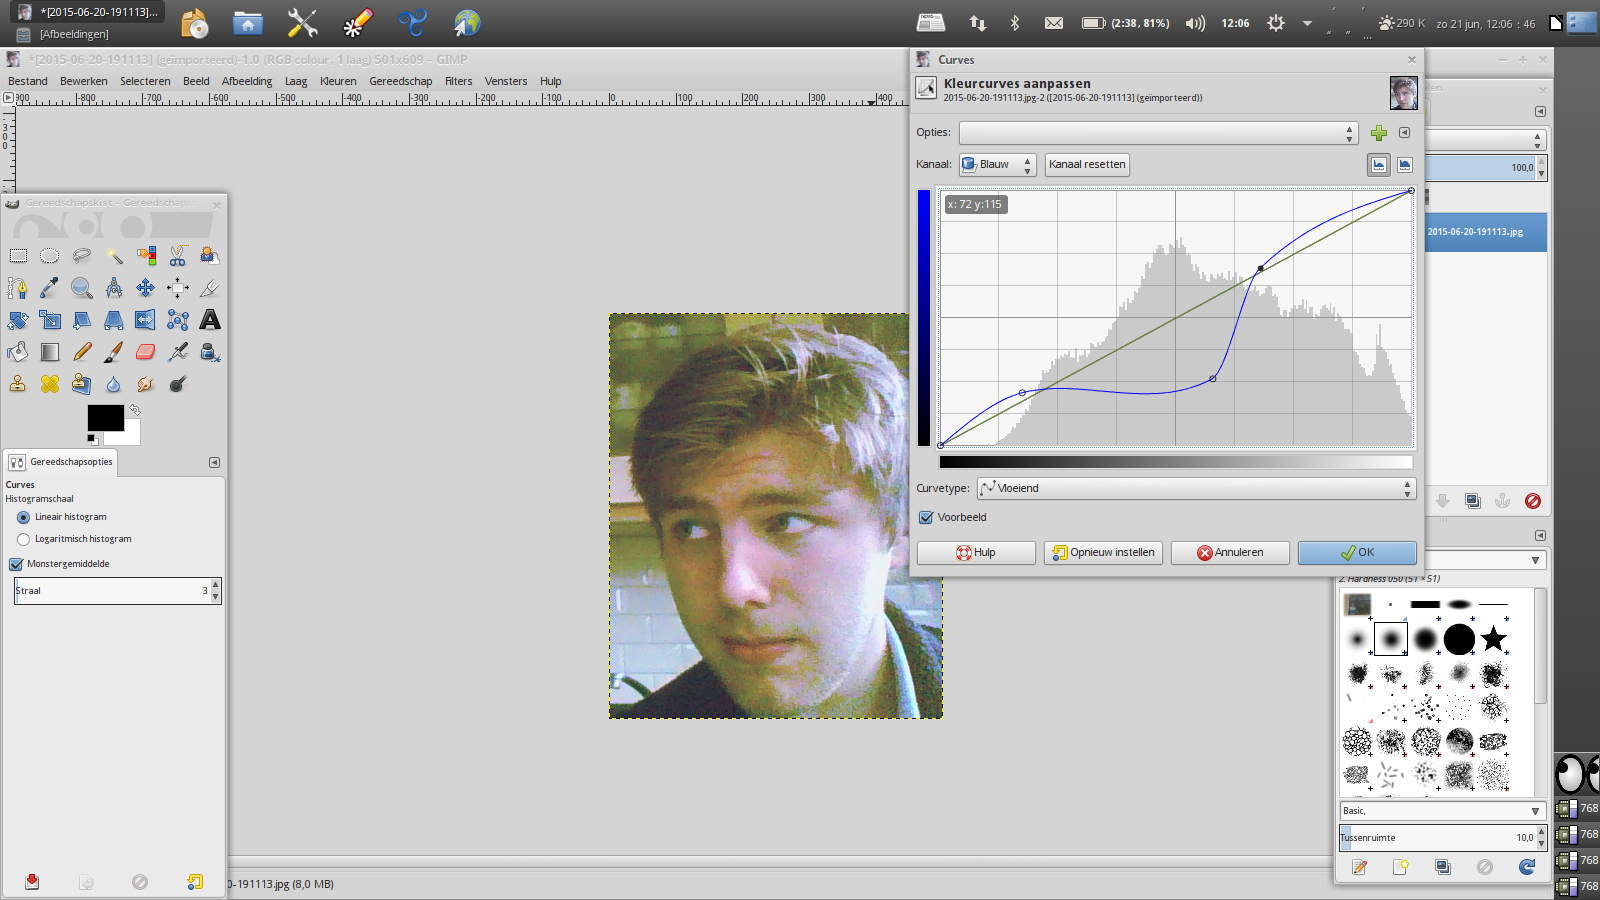
\includegraphics[width=1\linewidth]{kleurcurves/2.png}
     \end{figure}
     \begin{itemize}
      \item[1.] Kies een kanaal.
      \item[2.] Klik op de curve en sleep om een punt te maken
       (als daar nog geen punt is) of te verhogen of te verlagen.
      \item[3.] Herhaal tot u tevreden bent.
     \end{itemize}
    \item[3.] Activeer √OK.
   \end{itemize}
  \subsectie{Draaien}
   Een veel voorkomend probleem bij foto’s is de \textit{draaiing}.
   \begin{figure}
    \centering
    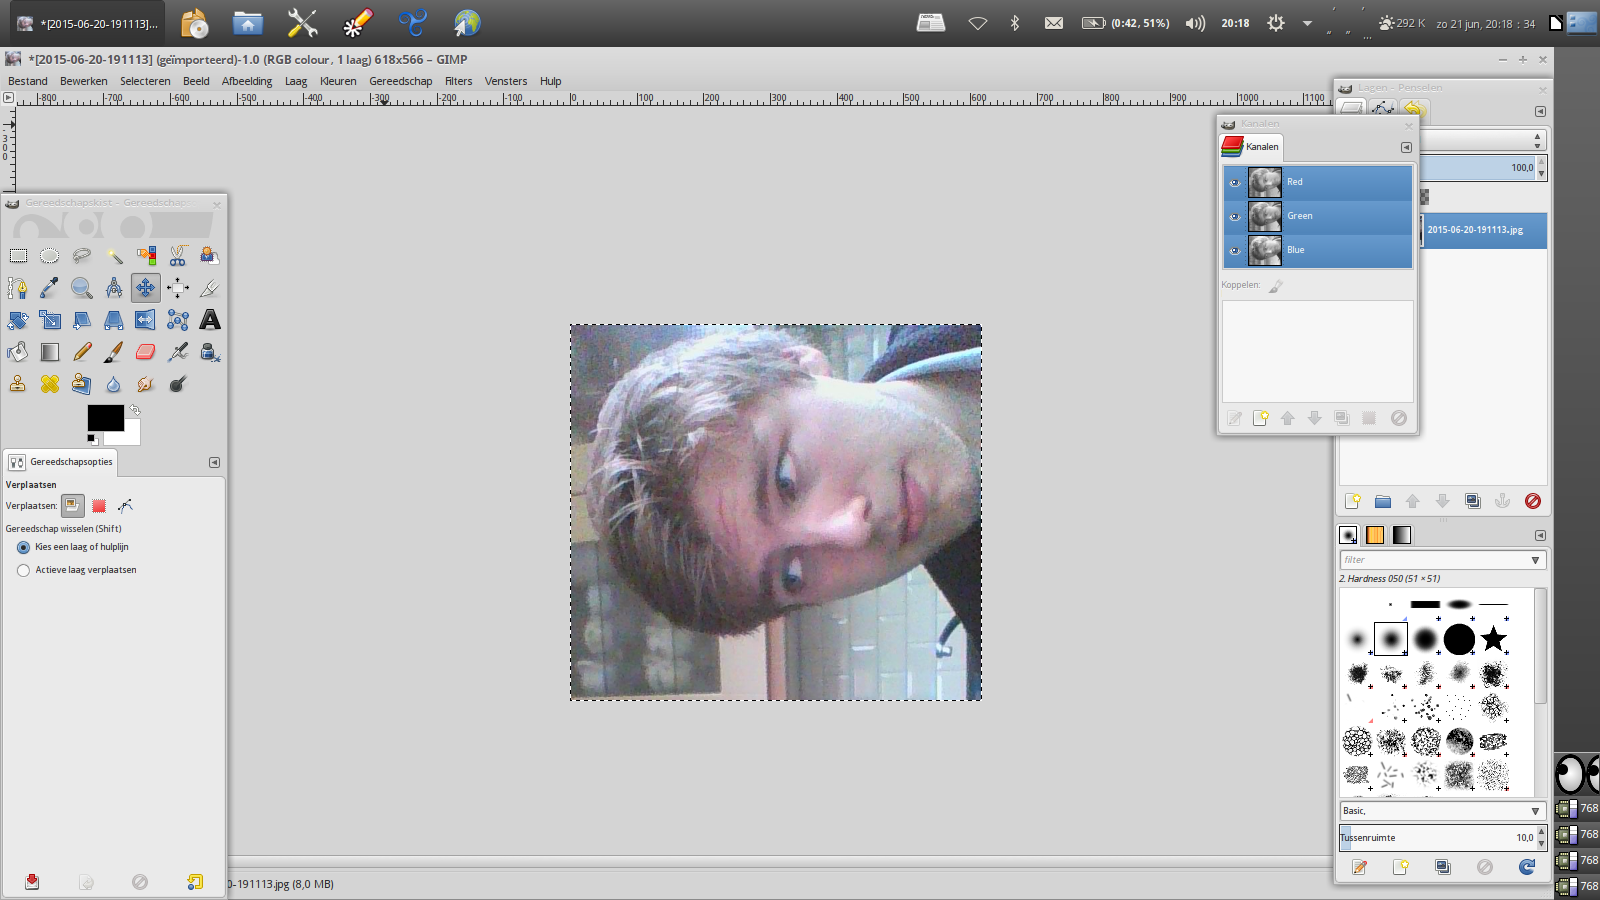
\includegraphics[width=1\linewidth]{draaien/1.png}
    \caption{gedraaide foto}
   \end{figure}
   Het gebeurt regelmatig dat afbeeldingen 90° te veel of te weinig
    gedraaid zijn. \GIMP{} kan gebruikt worden om deze afbeeldingen
    te herdraaien.
   \begin{itemize}
    \item[1.] Activeer, afhankelijk van het gewenste resultaat een van
     de menu-items onder ‘Afbeelding>Transformeren’: 90° met de klok
     mee draaien, 90° tegen de klok in draaien of 180° draaien.
   \end{itemize}
 \sectie{Foto’s oppeppen}\label{ding:oppepper}
  Als u een foto bewerkt, wilt u wellicht meer veranderen dan rimpeltjes,
   kleuren en rode ogen. Zo kunt u het ‘postereffect’ toepassen op foto’s
   voor posters. Of mischien wilt u ervoor zorgen dat het lijkt dat u geen
   foto’s hebt gemaakt, maar dat er een getekend hebt met olieverf!
  Al deze ‘oppeppers’ zijn mogelijk met \GIMP{}.
  \subsectie{Posterkleuren}\label{ding:posterkleuren}\label{ding:postereffect}
   Het postereffect bevindt zich in \GIMP{} niet in de categorie effecten.
   Het bevindt zich wel in het menu-item ‘Kleuren>Posterkleuren…’\\
   De slider posterkleurenniveaus bepaalt het aantal kleurenniveaus zoals
    u kunt zien in figuur \begin{figure}
     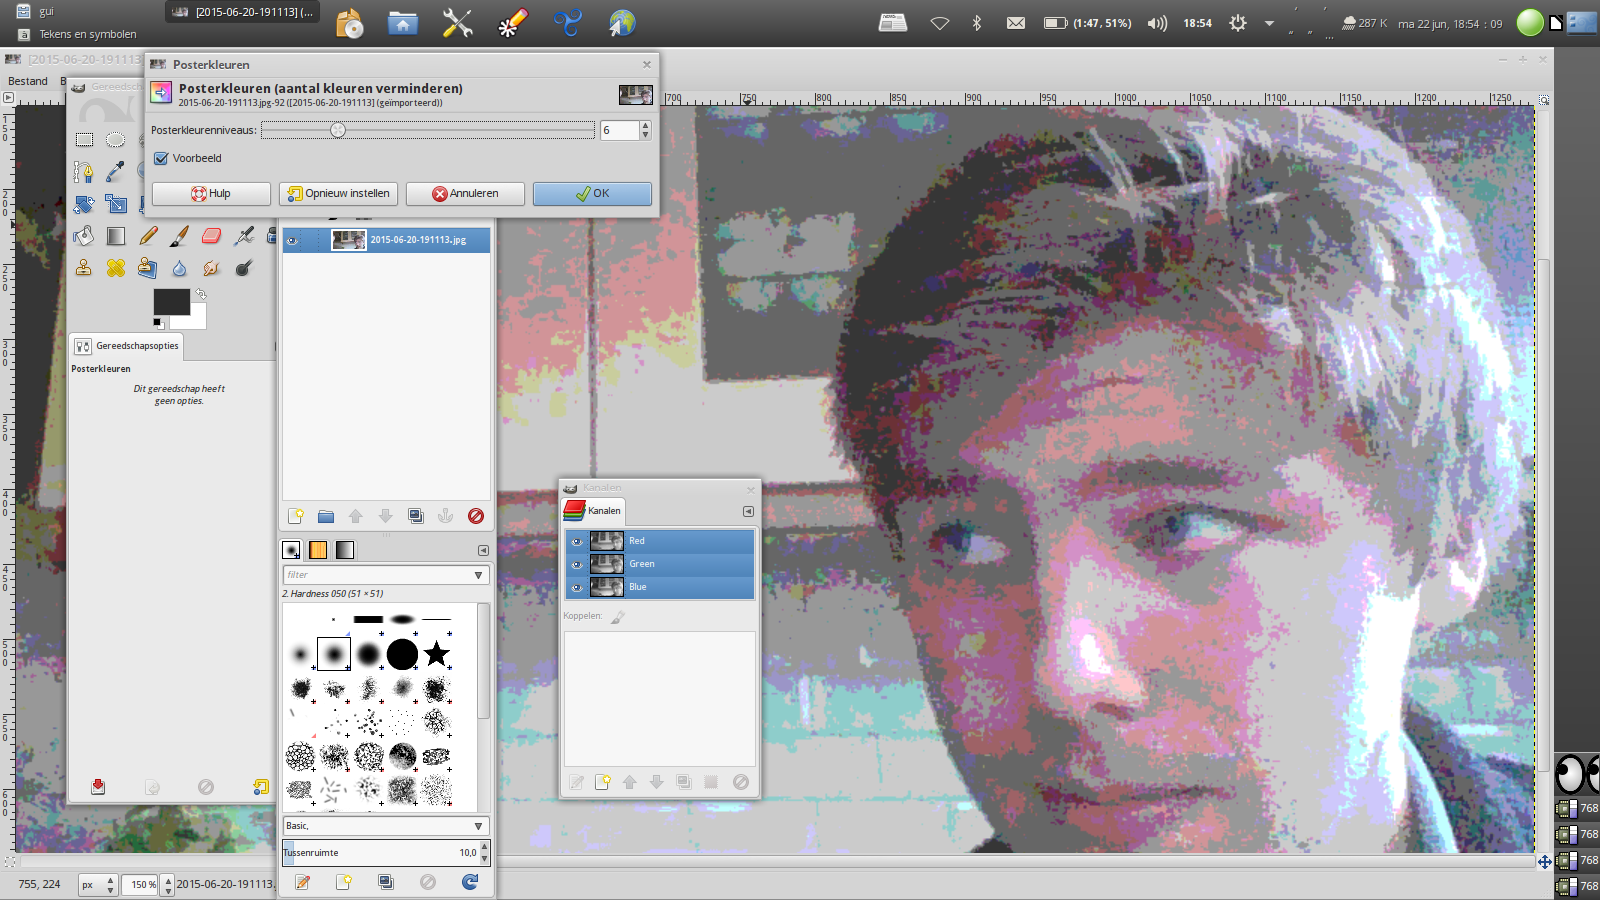
\includegraphics[width=0.90\linewidth]{oppepper/poster.png}
     \caption{het postereffect}
     \label{gx:poster}
    \end{figure}\ref{gx:poster}.
  \subsectie{Olieverf}\label{ding:olieverf}
   Olieverf bootst een olieverfschilderij na. U kunt het vinden onder
    Filters>Artistiek>Olieverf… Een grotere maskergrootte betekent een dikker
    penseel. Zie figuur \begin{figure}
     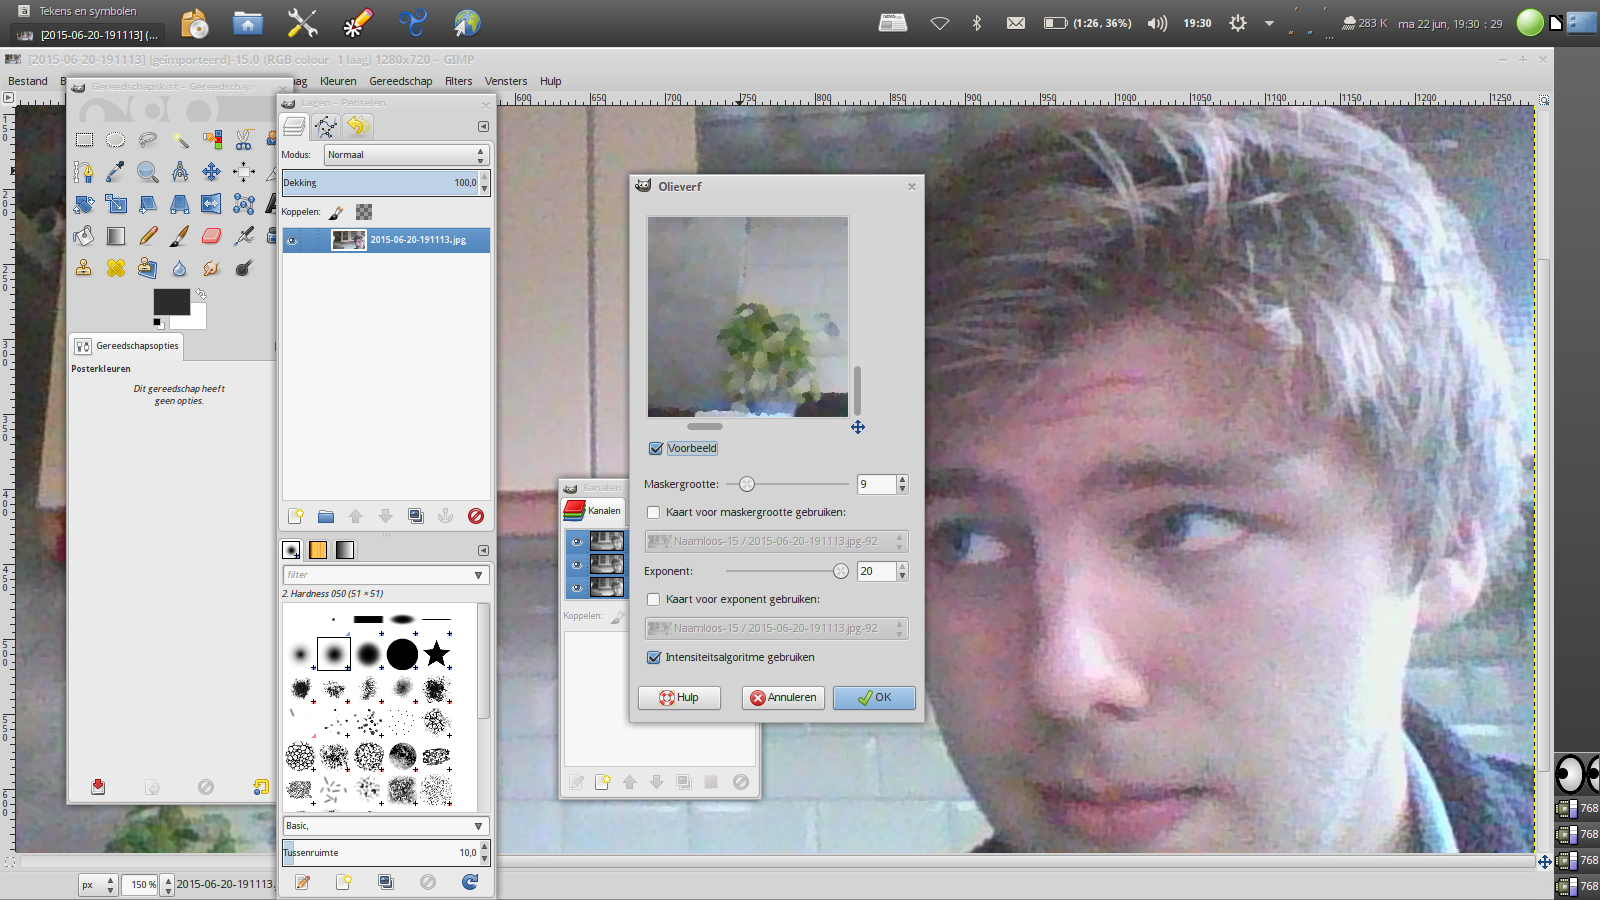
\includegraphics[width=0.90\linewidth]{oppepper/olieverf.png}
     \caption{olieverfschilderij}
     \label{gx:olieverf}
    \end{figure}\ref{gx:olieverf}.
  \subsectie{Kubisme}\label{ding:kubisme}
   \begin{center}
    kubisme: kubus + isme
   \end{center}
   Met het effect kubisme (\begin{figure}
    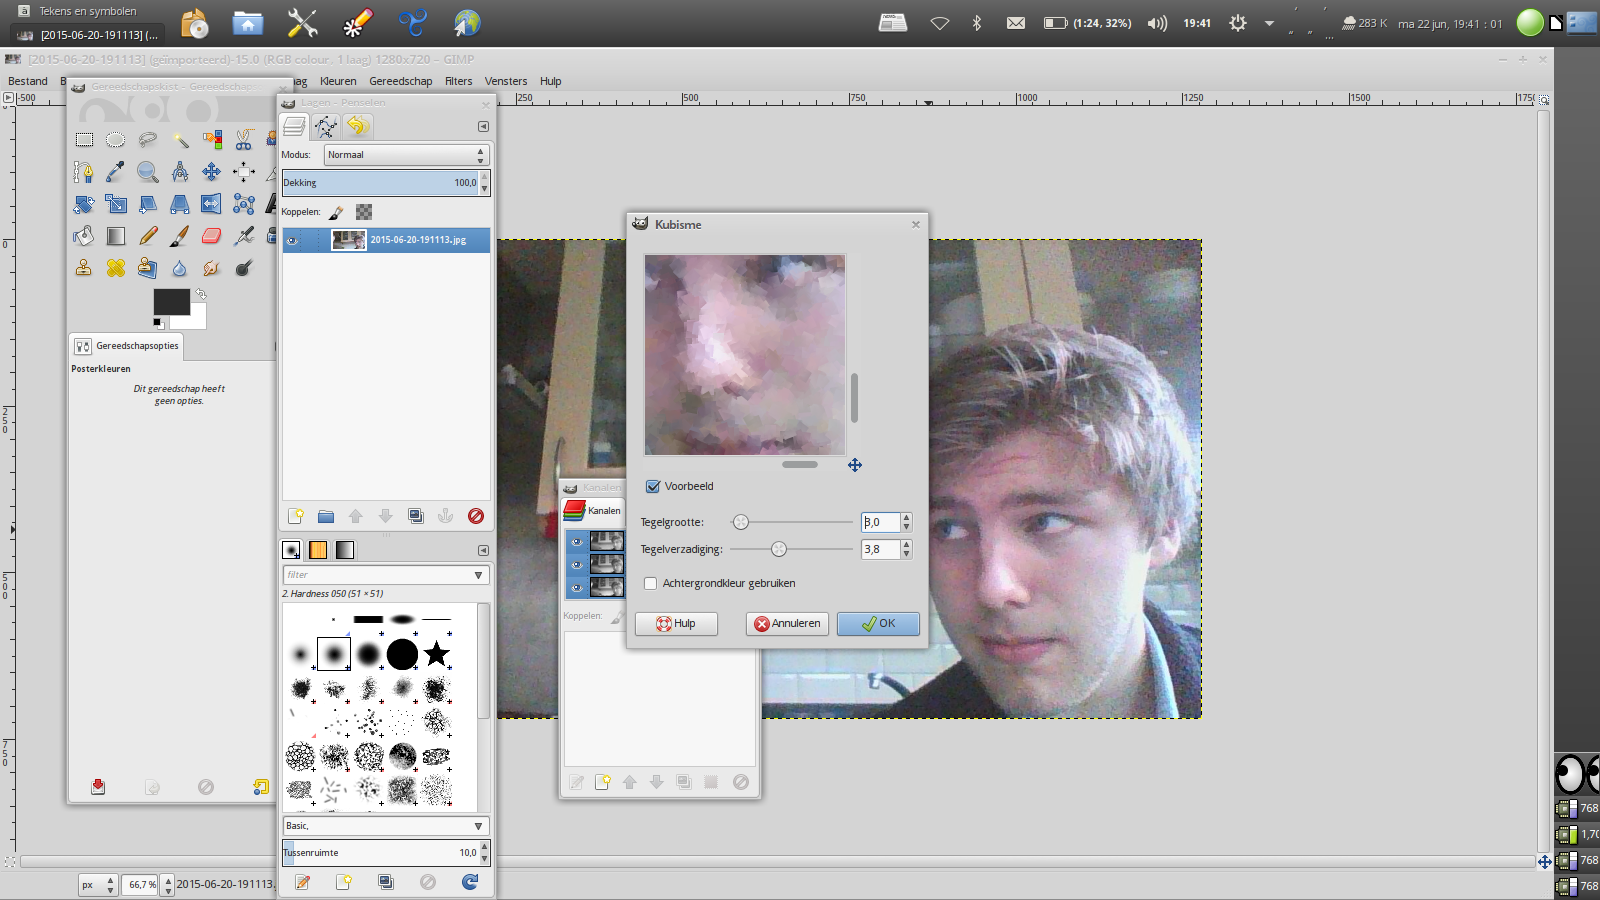
\includegraphics[width=0.90\linewidth]{oppepper/kubisme.png}
    \caption{kubisme}%
    \label{gx:kubisme}
   \end{figure}\ref{gx:kubisme}) wordt de afbeelding opnieuw getekend met
    vierkanten.
  \subsectie{Striptekening}\label{ding:striptekening}
   Striptekening laat de afbeelding eruit als een strip door de randen te
    benadrukken. \begin{figure}
     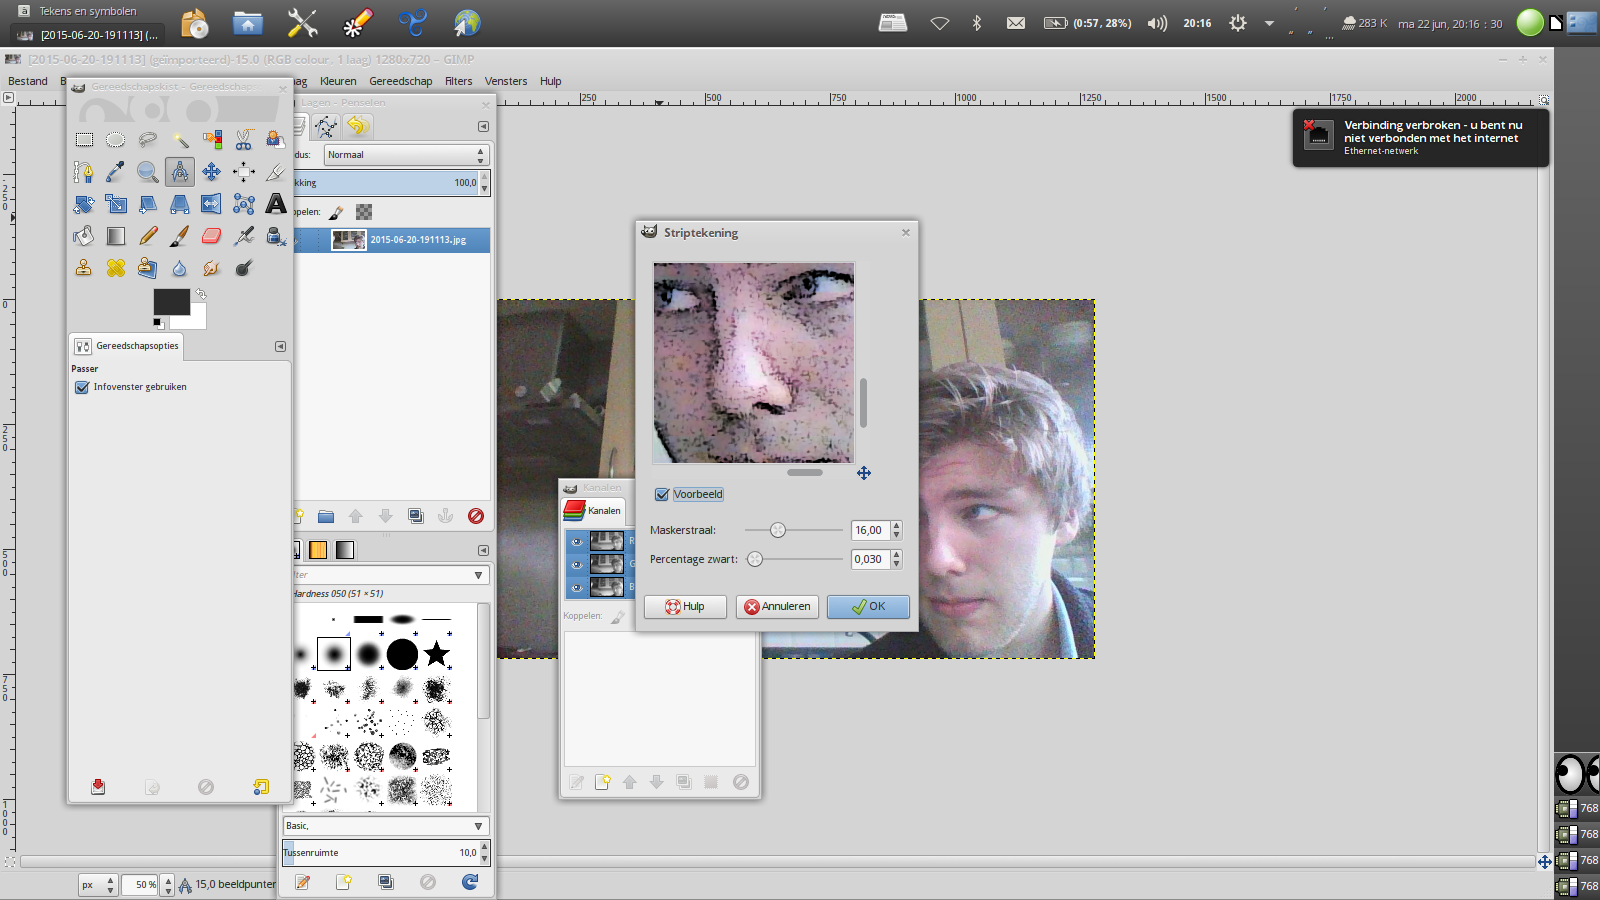
\includegraphics[width=0.90\linewidth]{oppepper/strip.png}
     \caption{striptekening}
     \label{gx:striptekening}
    \end{figure}
  \subsectie{Gloed}\label{ding:gloed}
   Gloed laat de afbeelding gloeien.
   \begin{figure}
    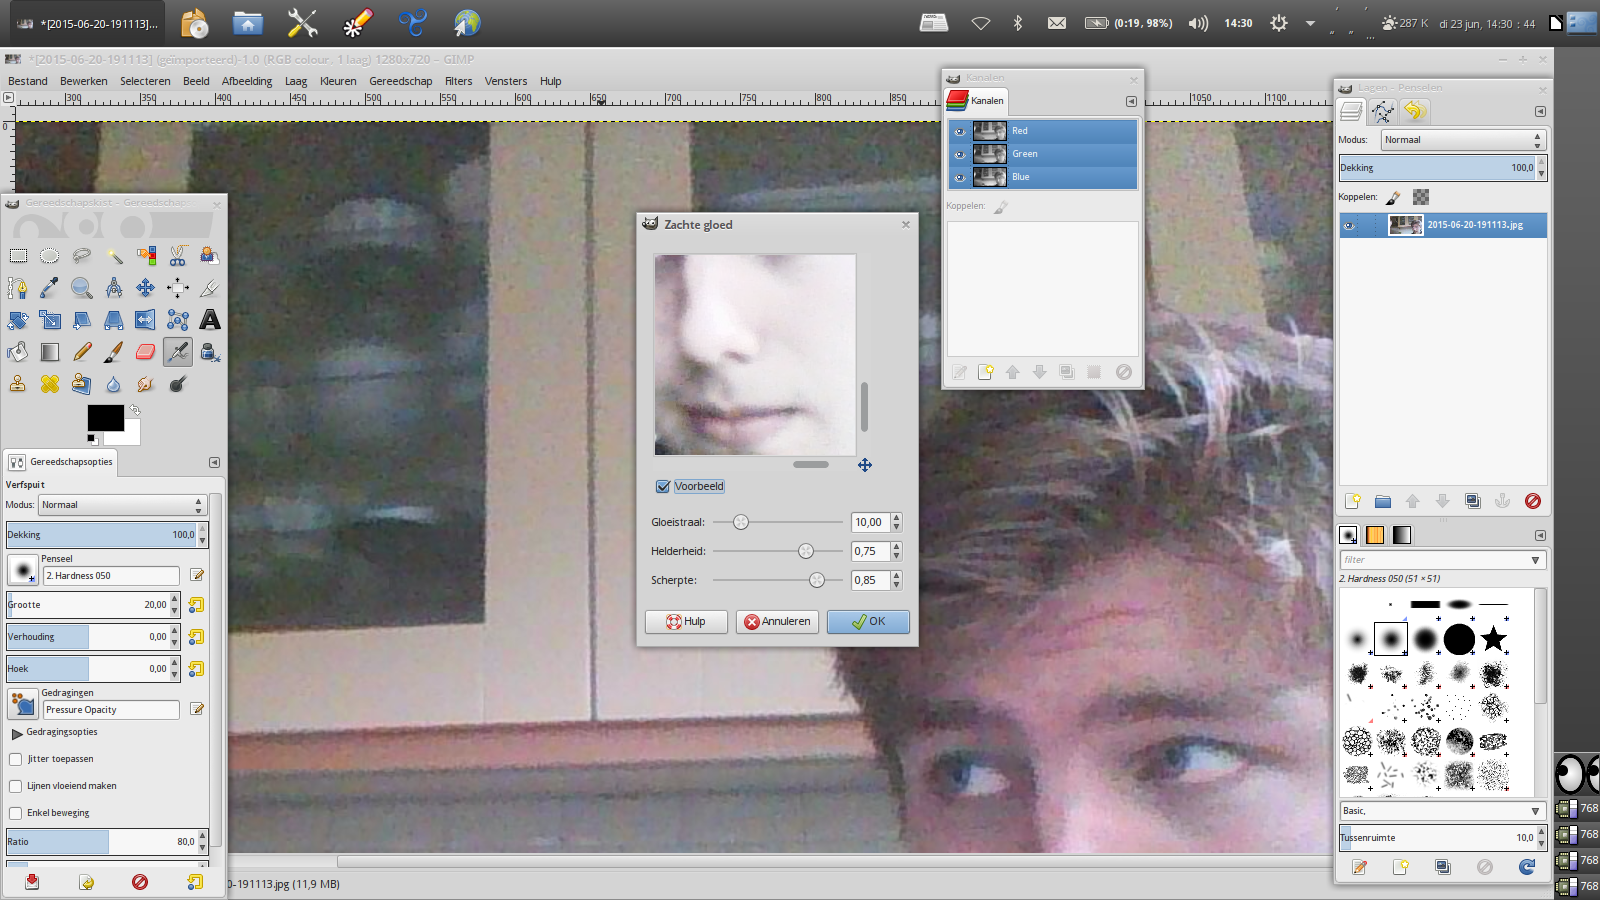
\includegraphics[width=0.9\linewidth]{oppepper/gloed.png}
    \caption{gloed}
    \label{gx:gloed}
   \end{figure}
\chapter{Gereedschappen}
 \sectie{Penselen}\label{ding:penseel}
  \GIMP{}’s tekengereedschappen gebruiken \textit{penselen}.
  Zo bestaat er een paprika-, pixel-, ster-, confetti, houtskool-,
   olie-, potlood-, rook-, zonne- en sponspenseel.
  \begin{figure}[btp]%
   \centering%
   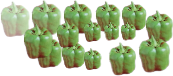
\includegraphics[width=0.49\linewidth]{gereedschappen/paprikafestijn.png}
   \includegraphics[width=0.49\linewidth]{gereedschappen/penseeleditor.pdf}
   \caption{paprika en de penselenbewerker}
   \label{gx:paprika}
  \end{figure} Deze penselen kunnen afbeeldingen zijn zoals in figuur
   \ref{gx:paprika}, maar ze kunnen ook cirkels, regelmatige sterren of 
    regelmatige veelhoeken zijn: ⭓⬛★⬤.
  \paragraph{}\label{ding:gum}\label{ding:potlood} Penselen gebruiken
   is eenvoudig. \GIMP{} heeft drie penseelgereedschappen:
   potlood, penseel en gum. De werkwijze is voor elk penseel
   hetzelfde.
  \begin{itemize}
   \item[1.] Activeer het gereedschap.
   \item[2.] Stel het gereedschap in. Een dekking lager dan 100 maakt
    het penseel doorzichtig, grootte verandert de grootte en met de
    penseelknop kunt u een penseel kiezen.
   \item[3.] Linkerklik op de afbeelding en versleep de muis terwijl u
    de linkermuisknop ingedrukt houdt.
  \end{itemize}
  \subsectie{Penselenbewerker}\label{ding:penselenbewerker}
   Met de penselenbewerker kunt u nieuwe regelmatige penselen
    aanmaken. Kies eerst de vorm, ⒜ cirkel, ⒝ vierkant of ⒞ diamant.
   Stel vervolgens de straal in. Verder kunt u ook het spakenaantal,
    de hardheid, de wit-zwartverhouding, de hoek en de tussenruimte
    veranderen. De tussenruimte is de ruimte tussen verschillende exemplaren
    van het penseel.
 \sectie{Selectie}\label{ding:selectie}
  \subsectie{Rechthoekig}
  \subsectie{Ovaalvormig}
   \GIMP{} heeft \textit{zeven} gereedschappen om selecties mee te manipuleren.
   De eenvoudigste zijn waarschijnlijk de rechthoekige en ovale. Deze
    werken op dezelfde manier: eerst klikt u op een uiterste punt van de grens en
    vervolgens sleept u dat naar een ander uiterste punt.
  \subsectie{Toverstaf}
   \includegraphics[height=4ex]{gereedschappen/toverstokkie.pdf}
   Er is niets magisch aan de toverstaf. De ‘toverstaf’ selecteerd de pixels
    met gelijkende kleuren die verbonden zijn met de oorspronkelijke via
    pixels met gelijkende kleuren.

   Door ‘Drempelwaarde’ te verhogen wordt de toverstaf toleranter,
    door het te verlagen wordt de staf kieskeuriger.
  \subsectie{Selecteren op kleur}
   \includegraphics[height=4ex]{gereedschappen/driekleur.pdf}
   De ‘driekleurenselectie’ selecteert de pixels met gelijkende kleuren.
   De opties zijn dezelfde als die van de toverstaf.
  \subsectie{De schaar}
   De schaar is een handig gereedschap om vormen mee te selecteren.
   \begin{itemize}
    \item[1.] Klik op een punt aan de rand van de vorm.
    \item[2.] Klik een punt dat een stukje verder ligt.
    \item[3.] Herhaal 2. totdat u aankomt bij een al geselecteerd punt.
    \item[4.] Klik op het eerste punt dat u selecteerde.
    \item[5.] Voltooi de selectie met ⏎.
   \end{itemize}
  \sectie{Pen}
   Zie \ref{ding:pen} (pag. \pageref{ding:pen}).
  \section{Pipet}
   Met het pipet kunt u kleuren ‘opzuigen’. U klikt op een pixel en voilà,
    de voorgrondkleur verandert! Met de controltoets wordt de achtegrondkleur
    in plaats van de voorgrondkleur ingesteld en de shifttoets laat een
    informatievenstertje verschijnen. Het venstertje bevat informatie over de
    kleur van de pixel.
  \sectie{Vergrootglas}
   Het vergrootglas vergroot of verkleint. Zonder control zoemt het in, met
    zoemt het uit.
  \sectie{Passer}
   De passer wordt gebruikt om afstanden en hoeken mee te meten.

   Kliksleep van het hoekpunt naar en uiteinde.

   Houdt, indien u een hoek wilt meten, vervolgens shift ingedrukt en
    kliksleep het hoekpunt naar het andere uiteinde.

   De afstand en de hoek staat in de statusbalk.
  \sectie{Bijsnijden}
   Kliksleep een rechthoek en gebruik ⏎. De afbeelding wordt dan beperkt
    tot de rechthoek.
  \sectie{Transformaties}
   \subsectie{Verplaatsen}
    Verplaatsen is in staat lagen, selecties en paden te verplaatsen.

    Kies eerst welk soort object u wilt verplaatsen. Is dit een laag, selectie
     of pad? Indien u een selectie verplaatst, verplaatst u alleen de selectie
     en niet de geselecteerde pixels.

    Kliksleep de selectie, het pad of de laag.
   \subsectie{Draaien}
    Draaien … draait.

    Draaien draait normaal gezien om het midden, maar dit kan aangepast worden.
    Klik op een punt en sleep het naar de gewenste nieuwe locatie. U kunt het
     draaipunt aanpassen door de cirkel met middellijnstukken te verplaatsen.
   \subsectie{Schalen}
    Schalen werkt zoals draaien, behalve dan dat het schaalt en de cirkel
     verplaatst. Indien de controltoets vastgehouden wordt, blijft de verhouding
     gelijk.
   \subsectie{Hellen}
    Hellen helt en werkt met kliksleep.
   \subsectie{Perspectief}
    Perspectief past perspectief toe.
    \begin{itemize}
     \item[1.] Klik op de afbeelding.
     \item[2.] Versleep de hoekpunten.
     \item[3.] ⏎
    \end{itemize}
   \subsectie{Spiegelen}
    Klik zonder control om horizontaal te spiegelen, met om verticaal te
     spiegelen. 
%   \subsectie{Transformeren}
%    te moeilijk om uit te leggen
\chapter{Paden}
 \section{Pen}\label{ding:pen}
\iffalse
\part{Scripten}
 \GIMP{} heeft uit\-ge\-brei\-de script\-ca\-pa\-ci\-teit\-en; zo zijn
  vod\-di\-fi\-ce\-ren, ver\-schil\-wol\-ken, lava en an\-de\-ren ge\-schre%
  \-ven als een script.
 De stukjes code die zullen komen, staan op de cd.
 \newcounter{Lijn}
 \newenvironment{bCode}[2]{%
  \\\rule{\linewidth}{0.4ex}%
  \begin{center}
   #2\hspace{4em}#1
  \end{center}
  \rule{\linewidth}{0.4ex}%
  \setlength\itemsep{1em}
  \begin{itemize}
   \ttfamily
  \setcounter{Lijn}{0}
  \newcommand{\lijn}{\stepcounter{Lijn}%
  \item[\theLijn>]}%
 }{%
  \end{itemize}%
  \rule{\linewidth}{0.8ex}
 }
 \begin{bCode}{eigenaardig.scm}{Wat zou deze code doen?}
  \lijn ; Wat zou dit doen?
  \lijn (define a (expt 2 3))
  \lijn (* a 2)
 \end{bCode}
 Om de voor\-beeld\-scripts uit te voeren, heeft u
  ‘Filters>Script-Fu>Server opstarten…’ nodig.
 \begin{figure}[h!]
  \centering
  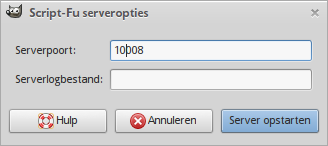
\includegraphics[width=0.9\linewidth]{script/server.png}
 \end{figure}
 Dat menu-item start een server
  op die bin\-nen\-komen\-de op\-dracht\-en uitvoert.
 We gaan ervanuit dat er bij Serverpoort 10008 staat.
 Let wel op: Script-Fu’s kunnen uw be\-stan\-den be\-wer\-ken!
 U kunt dus best tijdelijk uw net\-werk\-ver\-bin\-ding ver\-bre\-ken.

 \section{Inhoudsopgave}
  {\Large \textbf{Scripten}}
  \begin{itemize}
   \item[0] Scheme? Zijn die om op te eten?\hfill %
    \textbf{\pageref{scr:Scheme?}}
   \item[1] Getallen en zo \hfill \textbf{\pageref{scr:getallen}}
   \item[2] Peren van appels scheiden \hfill \textbf{\pageref{scr:peren}}
   \item[3] Opdrachten delegeren \hfill \textbf{\pageref{scr:delegeren}}
    \begin{itemize}
     \item[3.1] In herhaling vallen \dotfill{} \textbf{\pageref{scr:herhalen}}
    \end{itemize}
  \end{itemize}
 \chapter{Scheme? Zijn die om op te eten?}\label{scr:Scheme?}
  Nee, {\bfseries \textit{\textsc{Scheme is {\huge geen voedsel}.
  Het vult de maag {\huge niet}. Op Scheme alleen kunt u {\huge niet leven.}}}}

  Nu dit misverstand uit de weg is geruimd kunnen we weer verder.
  \begin{figure}
   \centering
   {\fontsize{140}{170}\selectfont λ}
   \caption{wat doet die lambda daar?}
  \end{figure} Om Script-Fu te kunnen gebruiken, moet men Scheme kennen.
  Om Scheme echt te kennen, moet men Scheme begrijpen.
  Scheme is een minimalistische taal. Functies kunnen opgeslagen worden
   in variabelen en loops worden gemaakt door staartrecursie.
  Scheme houdt van haken.
  \begin{bCode}{Breien.scm}{Haken? Breien!}
   \lijn (define (brei x) (expt x 2))
   \lijn (brei 8)
  \end{bCode}
  In vergelijking met andere talen zoals C, C++ en Java worden de accolades
   (\verb+{}+) niet gebruikt.
  \begin{longtabu} to \linewidth {|X[1,j] | X[7,j]|}\hline
   \multicolumn{2}{|c|}{Basissyntaxtekens}\\\hline
   teken     &  actie\\\hline
   ;         &  opmerking starten\newline
    De opmerking eindigt op het einde van de lijn.\\
   (         & groep beginnen\newline
    Beweringen gebruiken ook haken.\\
   )         & groep beëindigen\\
   \hline
  \end{longtabu}
 \chapter{Getallen en zo}\label{scr:getallen}%+-\
  \section{Letterdraden}
 \chapter{Peren van appels scheiden}\label{scr:peren}%if
 \chapter{Opdrachten delegeren}\label{scr:delegeren}%lambda
  \sectie{In herhaling vallen}\label{scr:herhalen}%recursie
\GIMP{}’s
  script\-taal heet Script-Fu en is ge\-ba\-seerd op Scheme.
\fi
\appendix{}
\chapter{‘Acknowledgements’ Erkenningen}
 In deze handleiding werden filters en fotomanipulaties botgevierd op
  een foto van een kennis. De auteur heeft er toestemming voor gekregen.
\chapter{GIMP helpen}
 Ook u kunt helpen met de ontwikkeling van \GIMP{}. U hebt daar geen speciaal
  talent voor nodig, al kan vriendelijk en beleefd zijn wel helpen.

 Zo kunt u \GIMP{} financieel steunen: met een donatie.
 \GIMP{}’s Bitcoinadres is \footnote{1NVMCeoBfTAJQ1qwX2Dx1C8zkcRCQWwHBq}. De
  ontwikkelaars van \GIMP{} kunnen uw \raisebox{-0.2ex}{%
   \includegraphics[width=1ex]{bitcoin.pdf}}’s goed gebruiken. De website van GIMP bevat informatie
  over andere manieren om te doneren: \footnote{%
   \BETEREURL{http://www.gimp.org/donating/}}.

 Verder kunt u, als kunt programmeren in C of Script-Fu,
  ook code schrijven voor \GIMP{}. Mischien vindt u wel
  een foutje in het programma.\footnote{%
  \BETEREURL{http://www.gimp.org/bugs/}%
 }

 U kunt ook documentatie schrijven.

 Kunst maken met \GIMP{} en die vervolgens verspreiden helpt zeker ook.
 Ten slotte kunt u ook \GIMP{} zelf verspreiden. Dat is volkomen legaal:
  het is vrije software! \GIMP{} maakt gebruik van de GNU General Public
  License.
 De laatste versie van de GNU GPL kan men vinden op \footnote{\BETEREURL{%
  https://www.gnu.org/licenses/gpl.html}}.
 Indien u een binaire versie verspreidt, moet men voldoen aan sectie 6:
  Conveying Non-Source Versions. U kunt daar eenvoudig aan voldoen door
  de broncode mee te geven op een medium dat geschikt is voor software%
  verspreiding\footnote{USB-stick, cd, dvd …}
\chapter{Deze handleiding aanpassen of verspreiden}
 Deze handleiding is een vrije handleiding en gebruikt de GNU Free Documentation
  License. De GNU FDL is een licentie voor vrije documentatie, net zoals de GNU GPL
  een licentie voor vrije software is. U mag deze handleiding verder verspreiden.

 De eenvoudige wijze om dat te doen is de handleiding afdrukken en de
  \XELATEX{}-bron code op een cd’tje of dergelijke meegeven. U mag hiervoor
  vergoeding vragen. 

 De auteur hoopt dat hij u niet moet uitleggen hoe u bestanden op opslagmedia moet zetten.
 \sectie{XeLaTeX 2. PDF}
 Om de code van het boek om te zetten in afdrukbare vorm hebt u een aantal computer%
  gereedschappen nodig:
 \begin{itemize}
  \item GNU Make 3.81
  \item GNU Coreutils
  \item GNU Sed
  \item GNU Grep
  \item \XELATEX{} en andere gerelateerde software, \TeX{}live van 14 juni 2014 is waarschijnlijk oké.
  \item FontForge 14:57 GMT 31-Jul-2012 (20120731-ML)
  \item Inkscape 0.48.4r9939
 \end{itemize}
 Mischien werken oudere versies; nieuwere versies werken waarschijnlijk ook.
 Om er PDF van te maken hoeft u dan slechts één opdracht uit te voeren:
 \texttt{make}\\
 Het PDF-bestand heet \texttt{gimp.pdf}. Indien u Ghostscript hebt staan op
  uw computer, kunt u de grootte beperken met\\
   \texttt{ghostscript -dBATCH -dNOPAUSE \textbackslash{}\\
   -sDEVICE=pdfwrite -dSubsetFonts=true \textbackslash{}\\
   -dCompressFonts \textbackslash{}\\
   -sOutputFile="Kleiner.pdf" \textbackslash{}\\
   gimp.pdf}
 \sectie{XeLaTeX}
 Deze handleiding werd geschreven in \LaTeX{} voor de \TeX{}-engine \XETEX{}.
 Er bestaan verschillende (Xe)(La)\TeX{} handleidingen: Wikibooks \LaTeX{},
  GNU TeX for the Impatient … \TeX{} uitleggen is buiten de context van deze
   handleiding.
 \sectie{Aanpassen}
  U moet de titel aanpassen, kies een titel die nog niet gebruikt is.
  In het begin van dit boek staan er een copyrightmededeling:


   Copyright © 2015 Maxime Devos.


  Plaats uw eigen copyrightmededeling erachter:

  \begin{longtabu}{c c l}
   Copyright ©&2015       &Maxime Devos.\\
   Copyright ©&HUIDIG JAAR&UW EIGEN NAAM.
  \end{longtabu}

  Nu moet u uw naam, het jaar, de nieuwe titel en de uitgever toevoegen
   aan de sectie ‘History’ Geschiedenis.

  Plaats op de titelpagina ten minste vijf (of alle, indien er niet vijf zijn)
   belangrijke auteurs. Vervang daar de uitgever door de nieuwe uitgever.
  Die kan dezelfde zijn.
  Behoudt de inhoud, toon en titel van de secties die Acknowledgements of
   Dedications in hun naam hebben.
  Verwijder de secties die Endorsements in hun naam hebben.
  Behoudt de copyrightmededelingen, de verantwoordelijkheidsdisclaimers
   en de inhoud van de sectie de History heet.
\begin{english}
\chapter{GNU Free Documentation License}
\begin{center}
 Version 1.3, 3 November 2008
 \setcounter{section}{-1}

 Copyright © 2000, 2001, 2002, 2007, 2008 Free Software Foundation, Inc.
     \BETEREURL{http://fsf.org/}\\
 Everyone is permitted to copy and distribute verbatim copies
 of this license document, but changing it is not allowed.
\end{center}

\nsectie{0. PREAMBLE}
The purpose of this License is to make a manual, textbook, or other
functional and useful document “free” in the sense of freedom: to
assure everyone the effective freedom to copy and redistribute it,
with or without modifying it, either commercially or noncommercially.
Secondarily, this License preserves for the author and publisher a way
to get credit for their work, while not being considered responsible
for modifications made by others.
\paragraph{}This License is a kind of “copyleft”, which means that derivative
works of the document must themselves be free in the same sense.  It
complements the GNU General Public License, which is a copyleft
license designed for free software.
\paragraph{}We have designed this License in order to use it for manuals for free
software, because free software needs free documentation: a free
program should come with manuals providing the same freedoms that the
software does.  But this License is not limited to software manuals;
it can be used for any textual work, regardless of subject matter or
whether it is published as a printed book.  We recommend this License
principally for works whose purpose is instruction or reference.
\nsectie{1. APPLICABILITY AND DEFINITIONS}
This License applies to any manual or other work, in any medium, that
contains a notice placed by the copyright holder saying it can be
distributed under the terms of this License.  Such a notice grants a
world-wide, royalty-free license, unlimited in duration, to use that
work under the conditions stated herein.  The “Document”, below,
refers to any such manual or work.  Any member of the public is a
licensee, and is addressed as “you”.  You accept the license if you
copy, modify or distribute the work in a way requiring permission
under copyright law.
\paragraph{}A “Modified Version” of the Document means any work containing the
Document or a portion of it, either copied verbatim, or with
modifications and/or translated into another language.
\paragraph{}A “Secondary Section” is a named appendix or a front-matter section of
the Document that deals exclusively with the relationship of the
publishers or authors of the Document to the Document’s overall
subject (or to related matters) and contains nothing that could fall
directly within that overall subject.  (Thus, if the Document is in
part a textbook of mathematics, a Secondary Section may not explain
any mathematics.)  The relationship could be a matter of historical
connection with the subject or with related matters, or of legal,
commercial, philosophical, ethical or political position regarding
them.
\paragraph{}The “Invariant Sections” are certain Secondary Sections whose titles
are designated, as being those of Invariant Sections, in the notice
that says that the Document is released under this License.  If a
section does not fit the above definition of Secondary then it is not
allowed to be designated as Invariant.  The Document may contain zero
Invariant Sections.  If the Document does not identify any Invariant
Sections then there are none.
\paragraph{}The “Cover Texts” are certain short passages of text that are listed,
as Front-Cover Texts or Back-Cover Texts, in the notice that says that
the Document is released under this License.  A Front-Cover Text may
be at most 5 words, and a Back-Cover Text may be at most 25 words.
\paragraph{}A “Transparent” copy of the Document means a machine-readable copy,
represented in a format whose specification is available to the
general public, that is suitable for revising the document
straightforwardly with generic text editors or (for images composed of
pixels) generic paint programs or (for drawings) some widely available
drawing editor, and that is suitable for input to text formatters or
for automatic translation to a variety of formats suitable for input
to text formatters.  A copy made in an otherwise Transparent file
format whose markup, or absence of markup, has been arranged to thwart
or discourage subsequent modification by readers is not Transparent.
An image format is not Transparent if used for any substantial amount
of text.  A copy that is not “Transparent” is called “Opaque”.
\paragraph{}Examples of suitable formats for Transparent copies include plain
ASCII without markup, Texinfo input format, \LaTeX{} input format, SGML
or XML using a publicly available DTD, and standard-conforming simple
HTML, PostScript or PDF designed for human modification.  Examples of
transparent image formats include PNG, XCF and JPG.  Opaque formats
include proprietary formats that can be read and edited only by
proprietary word processors, SGML or XML for which the DTD and/or
processing tools are not generally available, and the
machine-generated HTML, PostScript or PDF produced by some word
processors for output purposes only.
\paragraph{}The “Title Page” means, for a printed book, the title page itself,
plus such following pages as are needed to hold, legibly, the material
this License requires to appear in the title page.  For works in
formats which do not have any title page as such, “Title Page” means
the text near the most prominent appearance of the work’s title,
preceding the beginning of the body of the text.
\paragraph{}The “publisher” means any person or entity that distributes copies of
the Document to the public.
\paragraph{}A section “Entitled XYZ” means a named subunit of the Document whose
title either is precisely XYZ or contains XYZ in parentheses following
text that translates XYZ in another language.  (Here XYZ stands for a
specific section name mentioned below, such as “Acknowledgements”,
“Dedications”, “Endorsements”, or “History”.)  To “Preserve the Title”
of such a section when you modify the Document means that it remains a
section “Entitled XYZ” according to this definition.
\paragraph{}The Document may include Warranty Disclaimers next to the notice which
states that this License applies to the Document.  These Warranty
Disclaimers are considered to be included by reference in this
License, but only as regards disclaiming warranties: any other
implication that these Warranty Disclaimers may have is void and has
no effect on the meaning of this License.
\nsectie{2. VERBATIM COPYING}
You may copy and distribute the Document in any medium, either
commercially or noncommercially, provided that this License, the
copyright notices, and the license notice saying this License applies
to the Document are reproduced in all copies, and that you add no
other conditions whatsoever to those of this License.  You may not use
technical measures to obstruct or control the reading or further
copying of the copies you make or distribute.  However, you may accept
compensation in exchange for copies.  If you distribute a large enough
number of copies you must also follow the conditions in section 3.
\paragraph{}You may also lend copies, under the same conditions stated above, and
you may publicly display copies.
\nsectie{3. COPYING IN QUANTITY}
If you publish printed copies (or copies in media that commonly have
printed covers) of the Document, numbering more than 100, and the
Document’s license notice requires Cover Texts, you must enclose the
copies in covers that carry, clearly and legibly, all these Cover
Texts: Front-Cover Texts on the front cover, and Back-Cover Texts on
the back cover.  Both covers must also clearly and legibly identify
you as the publisher of these copies.  The front cover must present
the full title with all words of the title equally prominent and
visible.  You may add other material on the covers in addition.
Copying with changes limited to the covers, as long as they preserve
the title of the Document and satisfy these conditions, can be treated
as verbatim copying in other respects.
\paragraph{}If the required texts for either cover are too voluminous to fit
legibly, you should put the first ones listed (as many as fit
reasonably) on the actual cover, and continue the rest onto adjacent
pages.
\paragraph{}If you publish or distribute Opaque copies of the Document numbering
more than 100, you must either include a machine-readable Transparent
copy along with each Opaque copy, or state in or with each Opaque copy
a computer-network location from which the general network-using
public has access to download using public-standard network protocols
a complete Transparent copy of the Document, free of added material.
If you use the latter option, you must take reasonably prudent steps,
when you begin distribution of Opaque copies in quantity, to ensure
that this Transparent copy will remain thus accessible at the stated
location until at least one year after the last time you distribute an
Opaque copy (directly or through your agents or retailers) of that
edition to the public.
\paragraph{}It is requested, but not required, that you contact the authors of the
Document well before redistributing any large number of copies, to
give them a chance to provide you with an updated version of the
Document.
\nsectie{4. MODIFICATIONS}
\paragraph{}You may copy and distribute a Modified Version of the Document under
the conditions of sections 2 and 3 above, provided that you release
the Modified Version under precisely this License, with the Modified
Version filling the role of the Document, thus licensing distribution
and modification of the Modified Version to whoever possesses a copy
of it.  In addition, you must do these things in the Modified Version:
\begin{itemize}
\item[A.]
   Use in the Title Page (and on the covers, if any) a title distinct
   from that of the Document, and from those of previous versions
   (which should, if there were any, be listed in the History section
   of the Document).  You may use the same title as a previous version
   if the original publisher of that version gives permission.
\item[B.]
   List on the Title Page, as authors, one or more persons or entities
   responsible for authorship of the modifications in the Modified
   Version, together with at least five of the principal authors of the
   Document (all of its principal authors, if it has fewer than five),
   unless they release you from this requirement.
\item[C.]
   State on the Title page the name of the publisher of the
   Modified Version, as the publisher.
\item[D.]
   Preserve all the copyright notices of the Document.
\item[E.]
   Add an appropriate copyright notice for your modifications
   adjacent to the other copyright notices.
\item[F.]
   Include, immediately after the copyright notices, a license notice
   giving the public permission to use the Modified Version under the
   terms of this License, in the form shown in the Addendum below.
\item[G.]
   Preserve in that license notice the full lists of Invariant Sections
   and required Cover Texts given in the Document’s license notice.
\item[H.]
   Include an unaltered copy of this License.
\item[I.]
   Preserve the section Entitled “History”, Preserve its Title, and add
   to it an item stating at least the title, year, new authors, and
   publisher of the Modified Version as given on the Title Page.  If
   there is no section Entitled “History” in the Document, create one
   stating the title, year, authors, and publisher of the Document as
   given on its Title Page, then add an item describing the Modified
   Version as stated in the previous sentence.
\item[J.]
   Preserve the network location, if any, given in the Document for
   public access to a Transparent copy of the Document, and likewise
   the network locations given in the Document for previous versions
   it was based on.  These may be placed in the “History” section.
   You may omit a network location for a work that was published at
   least four years before the Document itself, or if the original
   publisher of the version it refers to gives permission.
\item[K.]
   For any section Entitled “Acknowledgements” or “Dedications”,
   Preserve the Title of the section, and preserve in the section all
   the substance and tone of each of the contributor acknowledgements
   and/or dedications given therein.
\item[L.]
   Preserve all the Invariant Sections of the Document,
   unaltered in their text and in their titles.  Section numbers
   or the equivalent are not considered part of the section titles.
\item[M.]
   Delete any section Entitled “Endorsements”.  Such a section
   may not be included in the Modified Version.
\item[N.]
   Do not retitle any existing section to be Entitled “Endorsements”
   or to conflict in title with any Invariant Section.
\item[O.]
   Preserve any Warranty Disclaimers.
\end{itemize}
\paragraph{}If the Modified Version includes new front-matter sections or
appendices that qualify as Secondary Sections and contain no material
copied from the Document, you may at your option designate some or all
of these sections as invariant.  To do this, add their titles to the
list of Invariant Sections in the Modified Version’s license notice.
These titles must be distinct from any other section titles.
\paragraph{}You may add a section Entitled “Endorsements”, provided it contains
nothing but endorsements of your Modified Version by various
parties — for example, statements of peer review or that the text has
been approved by an organization as the authoritative definition of a
standard.
\paragraph{}You may add a passage of up to five words as a Front-Cover Text, and a
passage of up to 25 words as a Back-Cover Text, to the end of the list
of Cover Texts in the Modified Version.  Only one passage of
Front-Cover Text and one of Back-Cover Text may be added by (or
through arrangements made by) any one entity.  If the Document already
includes a cover text for the same cover, previously added by you or
by arrangement made by the same entity you are acting on behalf of,
you may not add another; but you may replace the old one, on explicit
permission from the previous publisher that added the old one.
\paragraph{}The author(s) and publisher(s) of the Document do not by this License
give permission to use their names for publicity for or to assert or
imply endorsement of any Modified Version.
\nsectie{5. COMBINING DOCUMENTS}
You may combine the Document with other documents released under this
License, under the terms defined in section 4 above for modified
versions, provided that you include in the combination all of the
Invariant Sections of all of the original documents, unmodified, and
list them all as Invariant Sections of your combined work in its
license notice, and that you preserve all their Warranty Disclaimers.
\paragraph{}The combined work need only contain one copy of this License, and
multiple identical Invariant Sections may be replaced with a single
copy.  If there are multiple Invariant Sections with the same name but
different contents, make the title of each such section unique by
adding at the end of it, in parentheses, the name of the original
author or publisher of that section if known, or else a unique number.
Make the same adjustment to the section titles in the list of
Invariant Sections in the license notice of the combined work.
\paragraph{}In the combination, you must combine any sections Entitled “History”
in the various original documents, forming one section Entitled
“History”; likewise combine any sections Entitled “Acknowledgements”,
and any sections Entitled “Dedications”.  You must delete all sections
Entitled “Endorsement”.
\nsectie{6. COLLECTIONS OF DOCUMENTS}
You may make a collection consisting of the Document and other
documents released under this License, and replace the individual
copies of this License in the various documents with a single copy
that is included in the collection, provided that you follow the rules
of this License for verbatim copying of each of the documents in all
other respects.
\paragraph{}You may extract a single document from such a collection, and
distribute it individually under this License, provided you insert a
copy of this License into the extracted document, and follow this
License in all other respects regarding verbatim copying of that
document.
\nsectie{7. AGGREGATION WITH INDEPENDENT WORKS}
A compilation of the Document or its derivatives with other separate
and independent documents or works, in or on a volume of a storage or
distribution medium, is called an “aggregate” if the copyright
resulting from the compilation is not used to limit the legal rights
of the compilation’s users beyond what the individual works permit.
When the Document is included in an aggregate, this License does not
apply to the other works in the aggregate which are not themselves
derivative works of the Document.
\paragraph{}If the Cover Text requirement of section 3 is applicable to these
copies of the Document, then if the Document is less than one half of
the entire aggregate, the Document’s Cover Texts may be placed on
covers that bracket the Document within the aggregate, or the
electronic equivalent of covers if the Document is in electronic form.
Otherwise they must appear on printed covers that bracket the whole
aggregate.
\nsectie{8. TRANSLATION}
\paragraph{}Translation is considered a kind of modification, so you may
distribute translations of the Document under the terms of section 4.
Replacing Invariant Sections with translations requires special
permission from their copyright holders, but you may include
translations of some or all Invariant Sections in addition to the
original versions of these Invariant Sections.  You may include a
translation of this License, and all the license notices in the
Document, and any Warranty Disclaimers, provided that you also include
the original English version of this License and the original versions
of those notices and disclaimers.  In case of a disagreement between
the translation and the original version of this License or a notice
or disclaimer, the original version will prevail.
\paragraph{}If a section in the Document is Entitled “Acknowledgements”,
“Dedications”, or “History”, the requirement (section 4) to Preserve
its Title (section 1) will typically require changing the actual
title.
\nsectie{9. TERMINATION}
You may not copy, modify, sublicense, or distribute the Document
except as expressly provided under this License.  Any attempt
otherwise to copy, modify, sublicense, or distribute it is void, and
will automatically terminate your rights under this License.
\paragraph{}However, if you cease all violation of this License, then your license
from a particular copyright holder is reinstated (a) provisionally,
unless and until the copyright holder explicitly and finally
terminates your license, and (b) permanently, if the copyright holder
fails to notify you of the violation by some reasonable means prior to
60 days after the cessation.
\paragraph{}Moreover, your license from a particular copyright holder is
reinstated permanently if the copyright holder notifies you of the
violation by some reasonable means, this is the first time you have
received notice of violation of this License (for any work) from that
copyright holder, and you cure the violation prior to 30 days after
your receipt of the notice.
\paragraph{} Termination of your rights under this section does not terminate the
licenses of parties who have received copies or rights from you under
this License.  If your rights have been terminated and not permanently
reinstated, receipt of a copy of some or all of the same material does
not give you any rights to use it.
\nsectie{10. FUTURE REVISIONS OF THIS LICENSE}
The Free Software Foundation may publish new, revised versions of the
GNU Free Documentation License from time to time.  Such new versions
will be similar in spirit to the present version, but may differ in
detail to address new problems or concerns.\\
See \BETEREURL{http://www.gnu.org/copyleft/}.
\paragraph{} Each version of the License is given a distinguishing version number.
If the Document specifies that a particular numbered version of this
License “or any later version” applies to it, you have the option of
following the terms and conditions either of that specified version or
of any later version that has been published (not as a draft) by the
Free Software Foundation.  If the Document does not specify a version
number of this License, you may choose any version ever published (not
as a draft) by the Free Software Foundation.  If the Document
specifies that a proxy can decide which future versions of this
License can be used, that proxy’s public statement of acceptance of a
version permanently authorizes you to choose that version for the
Document.
\nsectie{11. RELICENSING}
“Massive Multiauthor Collaboration Site” (or “MMC Site”) means any
World Wide Web server that publishes copyrightable works and also
provides prominent facilities for anybody to edit those works.  A
public wiki that anybody can edit is an example of such a server.  A 
“Massive Multiauthor Collaboration” (or “MMC”) contained in the site
means any set of copyrightable works thus published on the MMC site.
\paragraph{} “CC-BY-SA” means the Creative Commons Attribution-Share Alike 3.0 
license published by Creative Commons Corporation, a not-for-profit 
corporation with a principal place of business in San Francisco, 
California, as well as future copyleft versions of that license 
published by that same organization.
\paragraph{} “Incorporate” means to publish or republish a Document, in whole or in 
part, as part of another Document.
\paragraph{} An MMC is “eligible for relicensing” if it is licensed under this 
License, and if all works that were first published under this License 
somewhere other than this MMC, and subsequently incorporated in whole or 
in part into the MMC, (1) had no cover texts or invariant sections, and 
(2) were thus incorporated prior to November 1, 2008.
\paragraph{} The operator of an MMC Site may republish an MMC contained in the site
under CC-BY-SA on the same site at any time before August 1, 2009,
provided the MMC is eligible for relicensing.
\nsectie{ADDENDUM: How to use this License for your documents}
\paragraph{} To use this License in a document you have written, include a copy of
the License in the document and put the following copyright and
license notices just after the title page:\\
\\
{\ttfamily
    Copyright (c)  YEAR  YOUR NAME.\\

    Permission is granted to copy, distribute and/or modify this document
    under the terms of the GNU Free Documentation License, Version 1.3
    or any later version published by the Free Software Foundation;
    with no Invariant Sections, no Front-Cover Texts, and no Back-Cover Texts.
    A copy of the license is included in the section entitled "GNU
    Free Documentation License".
}
\paragraph{} If you have Invariant Sections, Front-Cover Texts and Back-Cover Texts,
replace the “with...Texts” line with this:\\\\
{
\ttfamily with the Invariant Sections being LIST THEIR TITLES, with the
    Front-Cover Texts being LIST, and with the Back-Cover Texts being LIST.
}
\paragraph{} If you have Invariant Sections without Cover Texts, or some other
combination of the three, merge those two alternatives to suit the
situation.
\paragraph{} If your document contains nontrivial examples of program code, we
recommend releasing these examples in parallel under your choice of
free software license, such as the GNU General Public License,
to permit their use in free software.
\end{english}
\chapter{Multiwoordenlijst}
 \newenvironment{WOORD}[2]{%
  \subsection*{#1}\label{w:#1¿#2}}{}
\newcommand{\WSEC}[1]{\section*{#1}}
\newcommand{\HLI}{\\\noindent\makebox[\linewidth]{\rule{\paperwidth}{0.4pt}}}
 \WSEC{A}
  \begin{WOORD}{afbeelding}{afbeeldingen}
    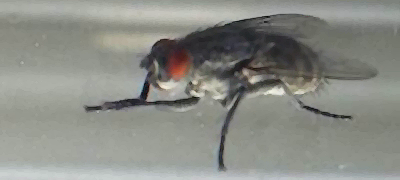
\includegraphics[width=\linewidth]{e/Sarcophaga_carnaria_(Portugal2005).png}
   Natuurlijk is afbeelding in de verzamelingenleer een
    interpretatie van het begrip functie, maar het woord
    heeft ook andere betekenissen.
   Een betekenis die waarschijnlijk bekender is, is een
    grafische representatie van een object.
  \end{WOORD}
% \WSEC{B}
% \WSEC{C}
% \WSEC{D}
% \WSEC{E}
% \WSEC{F}
 \WSEC{G}
  \begin{WOORD}{GIF}{GIF’s}
   GIF is een gelimiteerd afbeeldingsformaat. Het gebruik hiervan wordt
    afgeraden.
  \end{WOORD}
  \begin{WOORD}{GIMP}{GIMP’en}
   GIMP is een vrije desktopapplicatie om afbeeldingen
    mee te bewerken. Het heeft een eigen scripttaal:
    Script-Fu. De naam is een acroniem voor GNU Image Manipulation
    Program. Het kan gebruikt worden als een eenvoudig tekenprogramma,
    een fotoverbeteraar, afbeeldingsamenvoeger en waarschijnlijk
    nog veel meer\footnote{\BETEREURL{http://www.gimp.org/about/introduction%
     .html}}.
  \end{WOORD}
  \begin{WOORD}{GNU}{GNU’s}
   \begin{figure}
    \centering
    
\includegraphics[width=0.8\linewidth]{e/levignu.png}
   \end{figure}
   GNU is een Unix-achtig besturingssysteem.
   UNIX-achtigen bestaan uit vele programma’s, zoals
    bibliotheken, spelletjes, ontwikkelgereedschappen
    en toepassingen. GNU is een recursief acronym voor GNU
    is Niet Unix. GNU is namelijk niet Unix. GNU wordt
    uitgesproken als g'noe, als één lettergreep.
   \paragraph{} Het programma dat in Unix-achtigen systeembronnen
    beheert, met de hardware communiceert en de processen uitvoert,
    wordt een kernel genoemd. GNU wordt vaak gebruikt met de
    kernel Linux, maar niet altijd. GNU’s kernel is de Hurd.
   \paragraph{} Hurd bestond al voor Linux gestart was. Vrijwilligers
    werken verder aan de Hurd omdat het een interresant technisch project
    is.\footnote{\BETEREURL{https://www.gnu.org/\#More-GNU}}
  \end{WOORD}
  \begin{WOORD}{GNU Free Documentation License}{GNU Free Documentation Licenses}
   De GNU Free Documentation License is een licentie voor vrije documentatie,
    bv. handleidingen.
   Het GNU Project heeft geen definitie van vrije software, maar als ze er wel
    een zouden hebben, zou die gelijkaardig zijn aan de definitie van vrije software.
   Handleidingen met deze licentie kunnen aangepast, verandert en verkocht
    worden. Deze handleiding gebruikt de GNU FDL.
  \end{WOORD}
  \begin{WOORD}{GUI}{GUI’s}
   \textit{graphical user interface}\\
    grafische gebruikerinterface\\
   Een grafische gebruikerinterface is een grafische interface tussen
    de computer en de gebruiker. Deze bevat elementen zoals knoppen,
    menu’s, tekstvakken, tabvensters, schuifinvoer  …

   Vroeger kende men geen grafische gebruikerinterfaces, maar men kende wel
    textuele interfaces. Deze waren gebaseerd op tekst. Vandaag de dag worden
    deze ook nog gebruikt, met name in terminalapplicaties.

   Dit boek werd geschreven met de terminalapplicatie GNU nano.
  \end{WOORD}
\HLI
% \WSEC{H}
% \WSEC{I}
 \WSEC{J}
  \begin{WOORD}{JPEG}{JPEG’s}
   JPEG is een \textit{lossless} afbeeldingsformaat voor foto’s.
  \end{WOORD}
% \WSEC{K}
 \WSEC{L}
  \begin{WOORD}{lossless}{/}
   zonder \textit{extra} kwaliteitsverlies\\
   De kleuren van foto’s kunnen niet opgeslagen worden zoals ze echt zijn,
    ze kunnen niet oneindig veel ruimte in beslag nemen. In plaats daarvan
    hebben ze een beperkte ‘resolutie’, bitdiepte. PNG heeft vaak een bitdiepte
    van 8 bits. In theorie zou het ook heel groot kunnen zijn; een kibibyte bevoorbeeld.

   In de praktijk wordt dat niet gedaan, vooral omdat het te veel ruimte in
    beslag neemt en ook omdat het onnodig is: foto’s zijn meestal bedoeld
    voor mensen en die nemen toch niet zoveel waar.

   Beperkte bitdiepte, zolang die niet erg beperkt is, wordt meestal niet
    beschouwt als extra kwaliteitsverlies.
  \end{WOORD}
% \WSEC{M}
% \WSEC{N}
% \WSEC{O}
\HLI
 \WSEC{P}
  \begin{WOORD}{PNG}{PNG’s}
   PNG is een \textit{lossless} afbeeldingsformaat.
  \end{WOORD}
  \begin{WOORD}{programmeertaal}{programmeertalen}
   Een programmeertaal is een computertaal waarin geprogrammeerd kan worden.
   De meeste ‒ indien niet alle ‒ processors begrijpen enkel machinetaal: machinetaal
    is binaire code die rechtstreeks door de machine, de processor uitgevoerd kan worden.\\
    10111010 01010101 01011101 01101001 01001011 00100100 10101010 10010110 … Een machinetaal
    werkt meestal slechts op één type processor. Bepaalde programmeertalen zoals C, C++ en
    een hoop assemblytalen worden omgezet naar machinetaal, dit proces heet compileren.
   Meerdere gecompileerde stukjes van programma’s samenvoegen heet linken.
  \end{WOORD}
% \WSEC{Q}
% \WSEC{R}
\HLI
 \WSEC{S}
  \begin{WOORD}{Script-Fu}{Script-Fu’s}
   Script-Fu is GIMP’s scripttaal. Script-Fu is gebaseerd op Scheme%
    \footnote{\BETEREURL{http://docs.gimp.org/nl/gimp-concepts-script-fu.html}}%
   . Script-Fu is niet de enige scripttaal waarmee GIMP gescript kan worden,
    Perl en Tcl worden ook ondersteunt met extenties.
  \end{WOORD}
  \begin{WOORD}{scripttaal}{scripttalen}
   Scripttalen zijn programmeertalen. Waar de grens tussen script- en niet-scripttalen ligt
    is niet altijd duidelijk. Wat wel duidelijk is, is dat scripttalen vaak niet rechtstreeks
    door de processor worden uitgevoerd. Ze hebben meestal slechts beperkte toegang tot
    systeemfuncties en het komt minder vaak voor dat ze crashen, tenzij er een tekort aan
    geheugen heerst. ⇾ Script-Fu
  \end{WOORD}
\HLI
 \WSEC{T}
  \begin{WOORD}{TeX}{TeX’en}
   \TeX{} is een documentencompiler die bedoeld is om
    typografie van hoge kwaliteit te produceren. \TeX{} is
    WUZINWUK: wat u ziet is niet wat u krijgt: het lijkt erg
    veel op een programmeertaal, het is eigenlijk ook een
    programmeertaal. De opdrachten staan tussen de tekst
    en niet omgekeerd. \TeX{}s wiskundige typografiekwali%
    teiten staat goed bekend.

   \TeX{} werd geschreven door geschreven door Donald Knuth.

   Een stukje \TeX{} met \LaTeX{} macro’s:
   \\
   \verb+Ik houd van \textit{cursieve} \TeX{}.+\\
   \verb+\LaTeX{} is een macropakket voor \TeX{}.+\\
   \\
   Deze \LaTeX{}-code zorgt voor ‘Ik houd van \textit{cursieve}
    \TeX{}. \LaTeX{} is een macropakket voor \TeX{}.’
   Dit boek gebruikt een uitbreiding van \TeX{} met \LaTeX{}:
    \mbox{X\raisebox{-0.5ex}{Ǝ}\LaTeX{}}.
  \end{WOORD}
% \WSEC{U}
\HLI
 \WSEC{V}
%  \begin{WOORD}{Verlieswaardig}{Verlieswaardigen}
%   Voor al uw Verlieswaardig-problemen: \verb+format c:+\\
%   Opgeruimd staat netjes!
%  \end{WOORD}
  \begin{WOORD}{vrije software}{/}
   Vrije software is software die vrij is. Het gaat om de vrijheid, niet
    om de prijs. Denk aan \textit{libre} in het Frans en andere talen en niet
    aan vrij van kosten. Het GNU Project heeft een definitie van vrije software%
    \footnote{\BETEREURL{https://www.gnu.org/philosophy/free-sw.html}}:
   \begin{itemize}
    \item[0.]
     De vrijheid om het programma te gebruiken voor elk doel.
    \item[1.]
     De vrijheid om de manier waarop het programma werkt te bestuderen, en om het aan te passen aan je behoeften.
     Beschikbaarheid van de broncode is hiervoor noodzakelijk
    \item[2.]
     De vrijheid om het programma te verspreiden, zodat je je naasten kan helpen.
    \item[3.]
     De vrijheid om het programma te verbeteren en te verspreiden, zodat de hele gemeenschap hier voordeel van heeft.
     Beschikbaarheid van de broncode is ook hiervoor noodzakelijk.
   \end{itemize}
  \end{WOORD}
% \WSEC{W}
%  \begin{WOORD}{Windows}{Windowsen}
%   ⇾ Verlieswaardig
%   %dows: derdepersoonenkelvoudeenvoudighedenvorm van dow
%   %dow: to be worth: waardig zijn
%  \end{WOORD}
% \WSEC{X}
% \WSEC{Y}
% \WSEC{Z}
\label{EINDE}
\end{document}
